% vim: set spell spelllang=en tw=100 et sw=4 sts=4 foldmethod=marker foldmarker={{{,}}} :

\documentclass[aspectratio=169,compress,10pt]{beamer}

\usepackage{tikz}
\usepackage{xcolor}
\usepackage{complexity}
\usepackage{hyperref}
\usepackage{microtype}
\usepackage{amsmath}                   % \operatorname
\usepackage{amsfonts}                  % \mathcal
\usepackage{amssymb}                   % \nexists
\usepackage[vlined]{algorithm2e} % algorithms
\usepackage{centernot}
\usepackage{listings}
\usepackage{csquotes}
\usepackage{fancyvrb}
\usepackage{bussproofs}
\usepackage{multicol}
\usepackage{booktabs}
\usepackage{mathtools}
\usepackage{pifont}
\usepackage{marvosym}
\usepackage{cancel}

\usepackage{holtexbasic}
\usepackage{environ}
\NewEnviron{holthmenv}{%
  \scalebox{1.0}{\begin{array}[t]{l}
  \BODY
  \end{array}}}
\newcommand{\us}{\_}
\renewcommand{\HOLTokenTurnstile}{\ensuremath{\vdash\!\!}}
\renewcommand{\HOLConst}[1]{\textsf{\small #1}}
\renewcommand{\HOLFieldName}[1]{\textsf{\small #1}}
\renewcommand{\HOLSymConst}[1]{\HOLConst{#1}}
\renewcommand{\HOLTyOp}[1]{\HOLConst{#1}}
\renewcommand{\HOLinline}[1]{\textsf{\ensuremath{#1}}}
\renewcommand{\HOLKeyword}[1]{\ensuremath{\mathsf{#1}}}
\renewcommand{\HOLTokenBar}{\ensuremath{\mathtt{|}}}
\renewcommand{\HOLTokenLeftrec}{\ensuremath{\langle\!|}}
\renewcommand{\HOLTokenRightrec}{\ensuremath{|\!\rangle}}
\renewcommand{\HOLTokenLsl}{\raisebox{.15em}{\ensuremath{}\scriptsize{\textless\rule{-0.1em}{0em}\textless}{}}}

\renewcommand{\HOLStringLitDG}[1]{\scalebox{0.9}{\texttt{"#1"}}}
\renewcommand{\HOLStringLit}[1]{\scalebox{0.9}{\texttt{"#1"}}}
\renewcommand{\HOLCharLit}[1]{\scalebox{0.9}{\#\texttt{"#1"}}}
\newcommand{\HOLcount}[1]{\HOLTokenLeftbrace{}\HOLConst{0}\HOLSymConst{,}\HOLConst{1}\HOLSymConst{,}\HOLConst{...}\HOLSymConst{,}#1\HOLSymConst{\ensuremath{-}}\HOLConst{1}\HOLTokenRightbrace{}}

\usefonttheme{professionalfonts}

\usetikzlibrary{shapes, arrows, shadows, calc, positioning, fit}
\usetikzlibrary{decorations.pathreplacing, decorations.pathmorphing, shapes.misc}
\usetikzlibrary{tikzmark, backgrounds}
\usetikzlibrary{trees, overlay-beamer-styles}

\tikzset{processarrow/.style={->, very thick, decorate, decoration={snake, post length=0.5mm}}}
\tikzset{brace/.style={decorate, decoration={brace}, very thick}}

\definecolor{uofguniversityblue}{rgb}{0, 0.219608, 0.396078}
\definecolor{uofgheather}{rgb}{0.356863, 0.32549, 0.490196}
\definecolor{uofgaquamarine}{rgb}{0.603922, 0.72549, 0.678431}
\definecolor{uofgslate}{rgb}{0.309804, 0.34902, 0.380392}
\definecolor{uofgrose}{rgb}{0.823529, 0.470588, 0.709804}
\definecolor{uofgmocha}{rgb}{0.709804, 0.564706, 0.47451}
\definecolor{uofgsandstone}{rgb}{0.321569, 0.278431, 0.231373}
\definecolor{uofgforest}{rgb}{0, 0.2, 0.129412}
\definecolor{uofglawn}{rgb}{0.517647, 0.741176, 0}
\definecolor{uofgcobalt}{rgb}{0, 0.615686, 0.92549}
\definecolor{uofgturquoise}{rgb}{0, 0.709804, 0.819608}
\definecolor{uofgsunshine}{rgb}{1.0, 0.862745, 0.211765}
\definecolor{uofgpumpkin}{rgb}{1.0, 0.72549, 0.282353}
\definecolor{uofgthistle}{rgb}{0.584314, 0.070588, 0.447059}
\definecolor{uofgrust}{rgb}{0.603922, 0.227451, 0.023529}
\definecolor{uofgburgundy}{rgb}{0.490196, 0.133333, 0.223529}
\definecolor{uofgpillarbox}{rgb}{0.701961, 0.047059, 0}
\definecolor{uofglavendar}{rgb}{0.356863, 0.301961, 0.580392}

% {{{ theme things
\useoutertheme[footline=authortitle]{miniframes}
\useinnertheme{rectangles}

\setbeamerfont{block title}{size={}}
\setbeamerfont{title}{size=\large,series=\bfseries}
\setbeamerfont{section title}{size=\large,series=\mdseries}
\setbeamerfont{author}{size=\normalsize,series=\mdseries}
\setbeamercolor*{structure}{fg=uofguniversityblue}
\setbeamercolor*{palette primary}{use=structure,fg=black,bg=white}
\setbeamercolor*{palette secondary}{use=structure,fg=white,bg=uofgcobalt}
\setbeamercolor*{palette tertiary}{use=structure,fg=white,bg=uofguniversityblue}
\setbeamercolor*{palette quaternary}{fg=white,bg=black}
\setbeamercolor{block body}{bg=structure!10}
\setbeamercolor{block title}{bg=structure,fg=white}
\setbeamertemplate{blocks}[rounded]
\setbeamercolor*{titlelike}{parent=palette primary}

\beamertemplatenavigationsymbolsempty
\setbeamersize{text margin left=0.5cm}
\setbeamersize{text margin right=0.5cm}

\setbeamertemplate{title page}
{
    \begin{tikzpicture}[remember picture, overlay]
        \node at (current page.north west) {
            \begin{tikzpicture}[remember picture, overlay]
                \fill [fill=uofguniversityblue, anchor=north west] (0, 0) rectangle (\paperwidth, -2.6cm);
            \end{tikzpicture}
        };

        \node (logo) [anchor=north east, shift={(-0.8cm,-0.2cm)}] at (current page.north east) {
            
\includegraphics[keepaspectratio=true,scale=0.5]{../../images/UoG_keyline.pdf}
        };

        \node (logo2) [anchor=north, below=0.2cm of logo.south] {
            
\includegraphics[keepaspectratio=true,scale=0.1]{../../images/RAEngWhite.pdf}
        };

        \coordinate (logos) at ($(logo.south)!0.5!(logo2.north)$);

        \node [anchor=west, xshift=0.8cm] at (current page.west |- logos) {
            \begin{minipage}{0.65\paperwidth}\raggedright
                {\usebeamerfont{title}\usebeamercolor[white]{}\inserttitle}\\[0.2cm]
                {\usebeamerfont{author}\usebeamercolor[white]{}\insertauthor}
            \end{minipage}
        };
    \end{tikzpicture}
}

\setbeamertemplate{section page}
{
    \begin{centering}
        \begin{beamercolorbox}[sep=12pt,center]{part title}
            \usebeamerfont{section title}\insertsection\par
        \end{beamercolorbox}
    \end{centering}
}

\newcommand{\frameofframes}{/}
\newcommand{\setframeofframes}[1]{\renewcommand{\frameofframes}{#1}}

\makeatletter
\setbeamertemplate{footline}
{%
    \begin{beamercolorbox}[colsep=1.5pt]{upper separation line foot}
    \end{beamercolorbox}
    \begin{beamercolorbox}[ht=2.5ex,dp=1.125ex,%
        leftskip=.3cm,rightskip=.3cm plus1fil]{title in head/foot}%
        {\usebeamerfont{title in head/foot}\insertshorttitle}%
        \hspace{0.22\textwidth}%
        {\usebeamerfont{author in head/foot}\insertshortauthor}%
        \hfill%
        {\usebeamerfont{frame number}\usebeamercolor[fg]{frame number}\insertframenumber~\frameofframes~\inserttotalframenumber}
    \end{beamercolorbox}%
    \begin{beamercolorbox}[colsep=1.5pt]{lower separation line foot}
    \end{beamercolorbox}
}

\makeatletter
\setbeamertemplate{mini frame}
{%
  \begin{pgfpicture}{0pt}{0pt}{.04cm}{.04cm}
    \pgfpathcircle{\pgfpoint{0.04cm}{0.04cm}}{0.04cm}
    \pgfusepath{fill,stroke}
  \end{pgfpicture}%
}
\setbeamertemplate{mini frame in current subsection}
{%
  \begin{pgfpicture}{0pt}{0pt}{.04cm}{.04cm}
    \pgfpathcircle{\pgfpoint{0.04cm}{0.04cm}}{0.04cm}
    \pgfsetfillcolor{section in head/foot.bg}
    \pgfusepath{fill,stroke}
  \end{pgfpicture}%
}

\setbeamersize{mini frame size=0.10cm, mini frame offset=0.06cm}
\makeatother

\makeatletter
\newenvironment{nearlyplainframe}[2][]{
    \def\beamer@entrycode{\vspace*{-\headheight}\vspace*{3pt}}
    \setbeamertemplate{headline}
    {%
        \begin{beamercolorbox}[colsep=1.5pt]{upper separation line head}
        \end{beamercolorbox}
        \begin{beamercolorbox}[ht=0.5ex,dp=0.125ex,%
            leftskip=.3cm,rightskip=.3cm plus1fil]{title in head/foot}%
        \end{beamercolorbox}%
        \begin{beamercolorbox}[ht=0.5ex,dp=0.125ex,%
            leftskip=.3cm,rightskip=.3cm plus1fil]{author in head/foot}%
        \end{beamercolorbox}%
        \begin{beamercolorbox}[colsep=1.5pt]{lower separation line head}
        \end{beamercolorbox}
        \vspace*{\headheight}
    }

    \setbeamertemplate{footline}
    {%
        \begin{beamercolorbox}[colsep=1.5pt]{upper separation line foot}
        \end{beamercolorbox}
        \begin{beamercolorbox}[ht=0.5ex,dp=0.125ex,%
            leftskip=.3cm,rightskip=.3cm plus1fil]{author in head/foot}%
        \end{beamercolorbox}%
        \begin{beamercolorbox}[ht=0.5ex,dp=0.125ex,%
            leftskip=.3cm,rightskip=.3cm plus1fil]{title in head/foot}%
        \end{beamercolorbox}%
        \begin{beamercolorbox}[colsep=1.5pt]{lower separation line foot}
        \end{beamercolorbox}
    }

    \begin{frame}[#1]{#2}
    }{
    \end{frame}
}
\makeatother

% }}}

\tikzstyle{state} = [inner sep=1pt]
\tikzstyle{infeasible} = [color=uofgpillarbox]
\tikzstyle{dominated} = [color=uofgcobalt]
\tikzstyle{backwards} = []
\tikzstyle{accept} = [solid, thick]
\tikzstyle{reject} = [dotted, thick]
\tikzstyle{forced} = [color=uofglawn]
\tikzstyle{domination} = [dashed, thick, ->, color=uofgcobalt]

\newcommand{\set}[1]{\{ #1 \}}
\newcommand{\setsize}[1]{{\left|#1\right|}}

\newcommand{\solvernameformat}[1]{\textit{#1}}
\newcommand{\toolformat}[1]{\textit{#1}}
\newcommand{\proofsystemformat}[1]{\textsc{#1}\@}

\newcommand{\veripb}{\toolformat{VeriPB}\xspace}
\renewcommand{\veripb}{\proofsystemformat{VeriPB}\xspace}
\newcommand\veripbid[1]{\alertred{#1}}
\newcommand\veripbConstraint[1]{\alertblue{#1}}

\newcommand{\neighbourhood}{\operatorname{N}}
\newcommand{\vertexset}{\operatorname{V}}
\newcommand{\degree}{\operatorname{deg}}

\providecommand{\reifvar}{r}
\providecommand{\reifimpllft}{\Leftarrow}
\providecommand{\reifimplrt}{\Rightarrow}
\providecommand{\reifequiv}{\Leftrightarrow}
\providecommand{\reifconstrlft}[2]{#1 \reifimpllft #2}
\providecommand{\reifconstrrt}[2]{#1 \reifimplrt #2}
\providecommand{\reifconstrequiv}[2]{#1 \reifequiv #2}

\newcommand{\colorblue}[1]{\textcolor{uofgcobalt}{#1}}
\newcommand{\colorred}[1]{\textcolor{uofgthistle}{#1}}
\newcommand{\colorgreen}[1]{\textcolor{uofglawn}{#1}}

% For highlighting in examples
%   \newcommand<>{\alertred}[1]{{\color#2{red}#1}}
\newcommand<>{\alertred}[1]{{\color#2{uofgthistle}#1}}
\renewcommand<>{\alert}[1]{{\color#2{uofgthistle}#1}}
%   \newcommand<>{\alertblue}[1]{{\color#2[rgb]{0,0,0.7}#1}}
\newcommand<>{\alertblue}[1]{{\color#2{uofgcobalt}#1}}
%   \newcommand<>{\alertgreen}[1]{{\color#2[rgb]{0,0.6,0}#1}}
\newcommand<>{\alertgreen}[1]{{\color#2{uofglawn}#1}}

%%% Extra alert command colours
\newcommand<>{\alertlav}[1]{{\color#2{uofglavendar}#1}}
% Pillarbox is kind of red
\newcommand<>{\alertpillarbox}[1]{{\color#2{uofgpillarbox}#1}}
% Pumpkin is kind of orange
\newcommand<>{\alertpumpkin}[1]{{\color#2{uofgpumpkin}#1}}
\newcommand<>{\alertorange}[1]{{\color#2{uofgpumpkin}#1}}

%%% White text to reserve right amount of space
\newcommand<>{\alertwhite}[1]{{\color#2{white}#1}}

\author{Ciaran McCreesh}
\title{Pseudo-Boolean Proof Logging for Problems that are not Pseudo-Boolean}

\begin{document}

{
    \usebackgroundtemplate{
        \tikz[overlay, remember picture]
        \node[at=(current page.south), anchor=south, inner sep=0pt, yshift=-1.4cm]{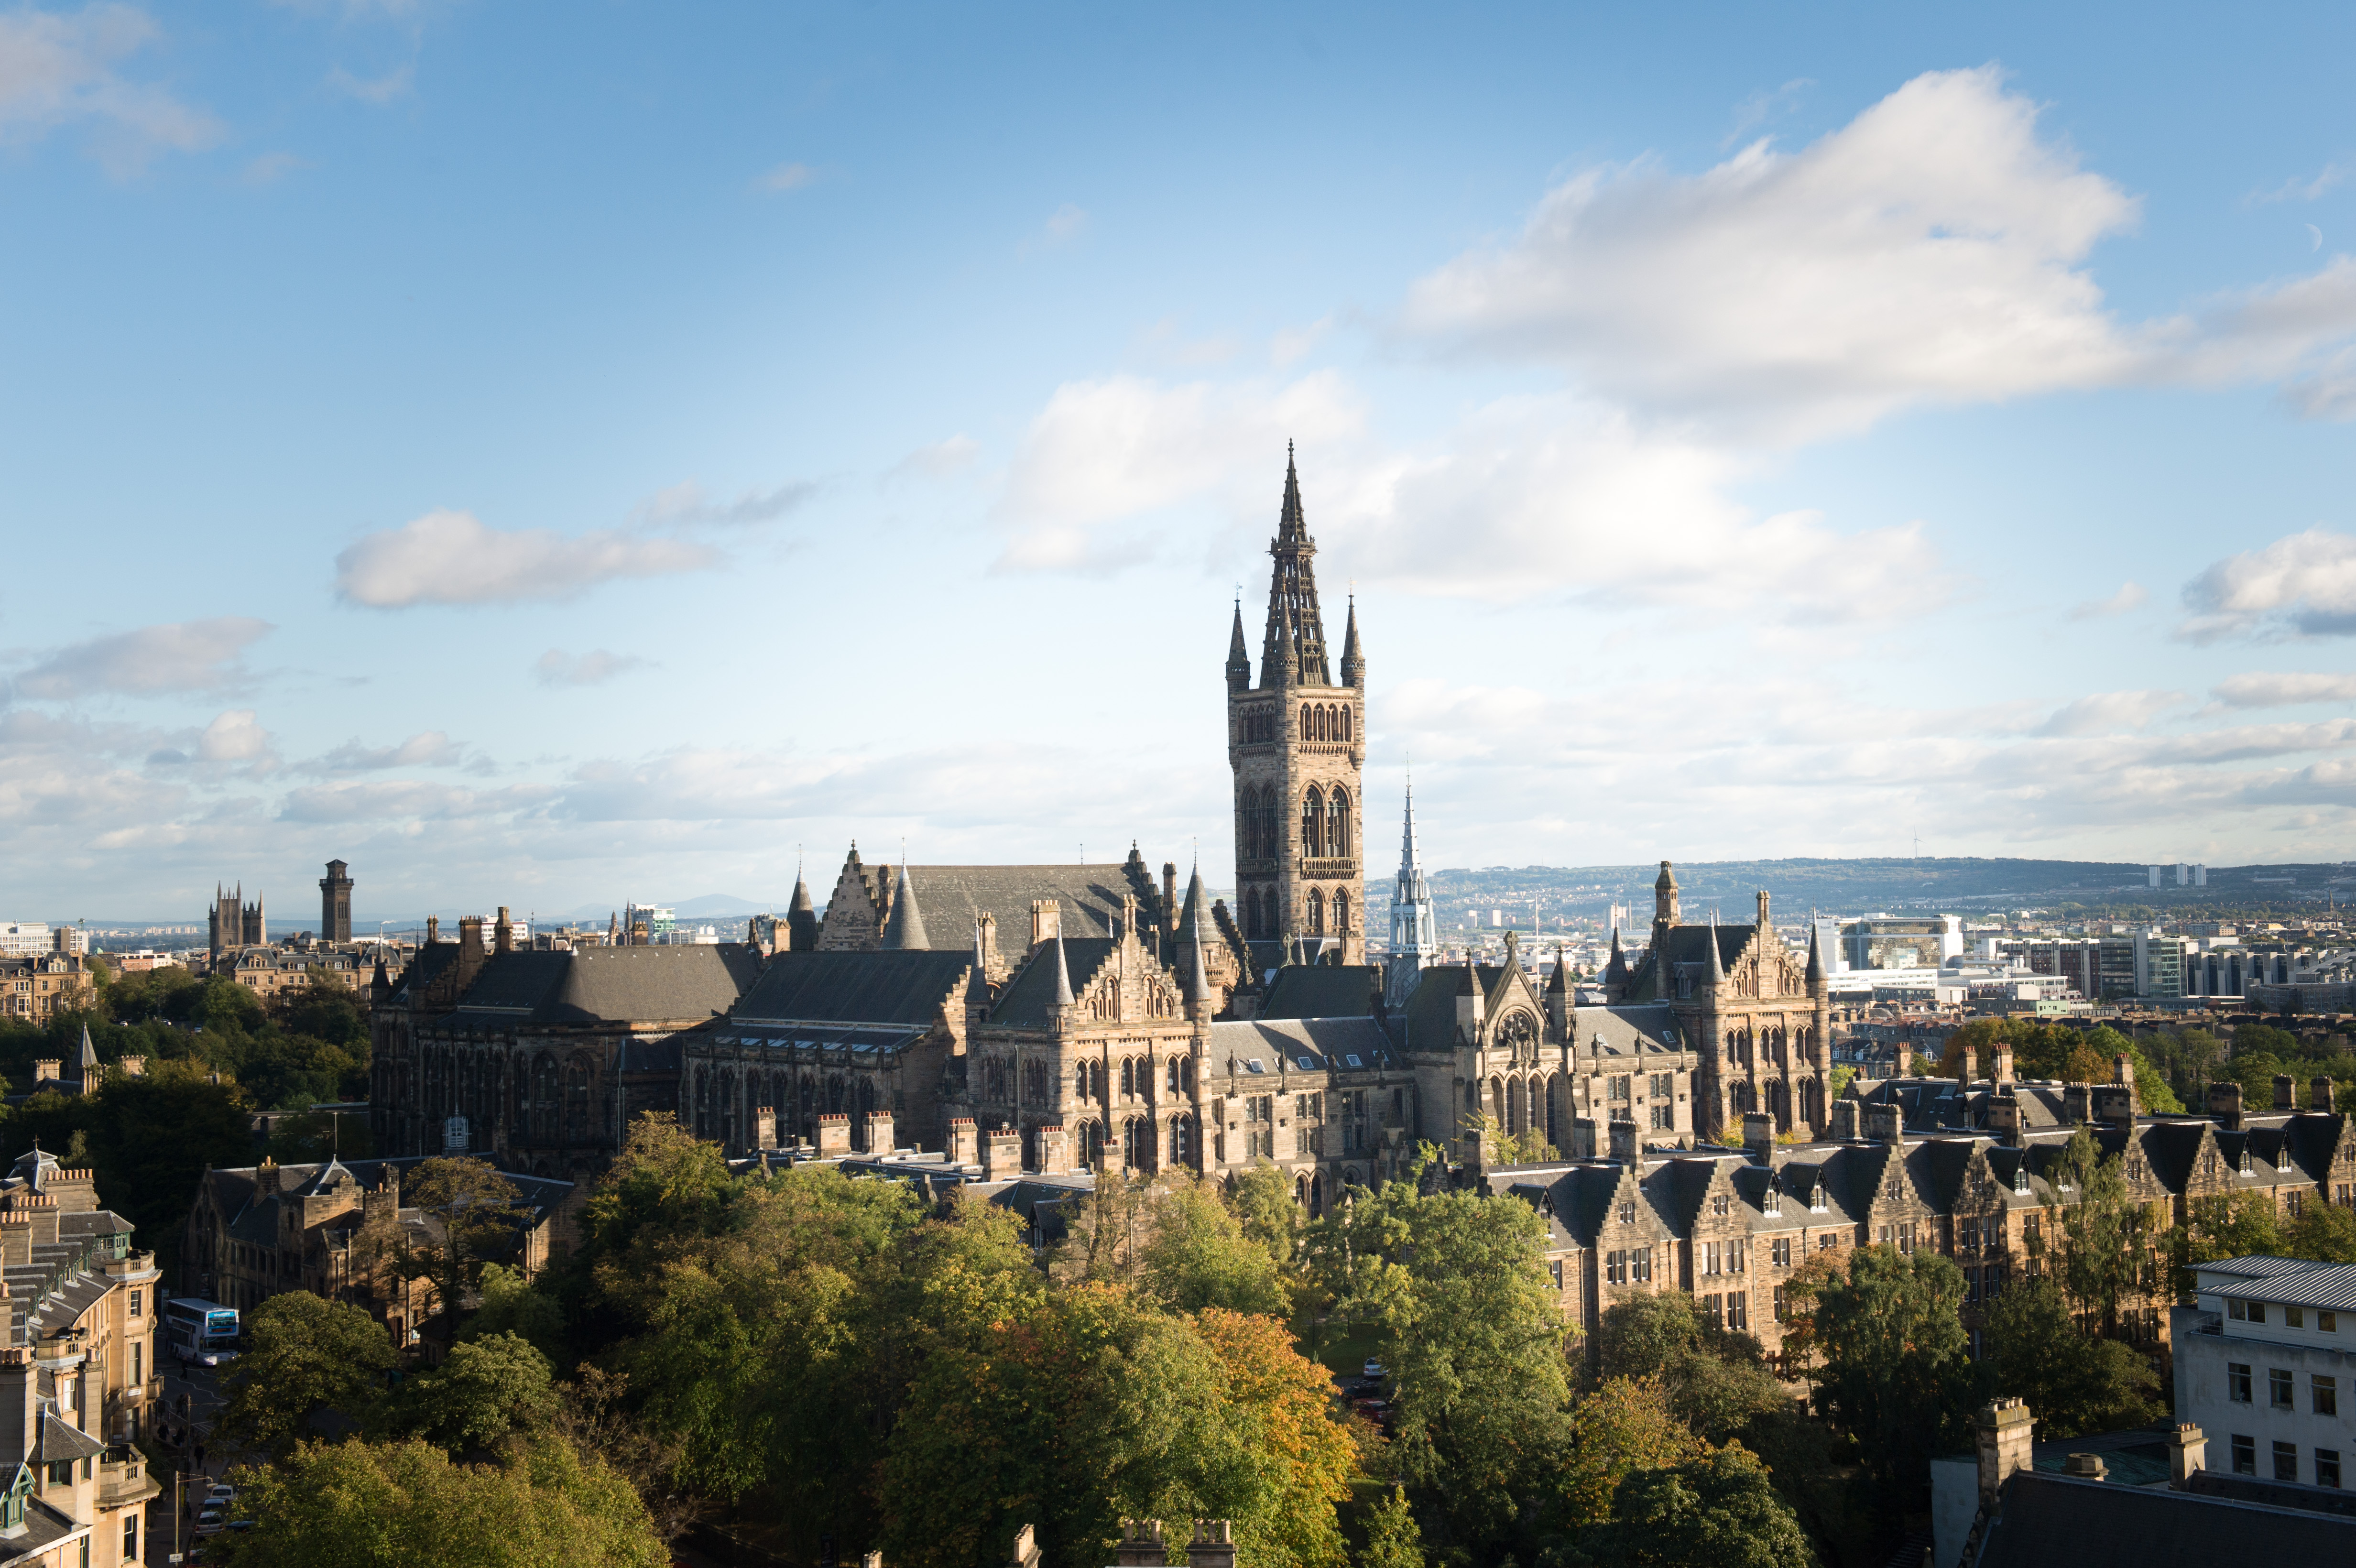
\includegraphics[keepaspectratio=true, width=\paperwidth]{../../images/background.jpg}};
    }
    \begin{frame}[plain,noframenumbering]
        \titlepage
    \end{frame}
}

\section{Recap}

\begin{frame}{Proof Logging}
    \vspace*{-1.0em}
    \begin{center}
        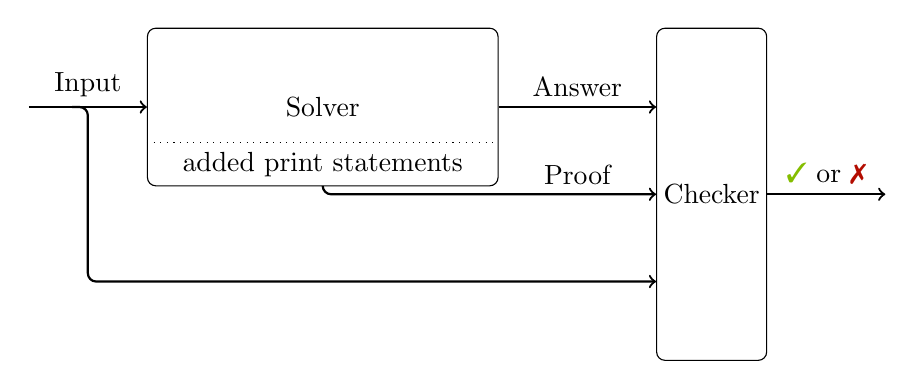
\begin{tikzpicture}
            \node (solver) [inner xsep=5em, inner ysep=2.5em, draw, rounded corners=3pt] { Solver };

            \node (checker) [right=2cm of solver.north east, anchor=north west, inner xsep=0.25em, draw, rounded corners=3pt, minimum height=12em, visible on=<3->] { Checker };

            \node (print) [anchor=south, above=0cm of solver.south, visible on=<2->] { added print statements };
            \draw [dotted, visible on=<2->] (solver.west|-print.north) -- (solver.east|-print.north);

            \draw [->, thick] (solver.east) -- (solver.east -| checker.west)
                coordinate [midway] (solutionmid) node [above, midway] { Answer };

            \draw [->, thick, rounded corners=3pt, visible on=<2->] (solver.south) -- (solver.south |- checker.west)
                -- (checker.west) coordinate [midway] (proofmid);

            \coordinate (prooflabel) at (proofmid-|solutionmid);
            \node [above=0cm of prooflabel, visible on=<2->] { Proof };

            \coordinate [right=1.5cm of checker.east] (verified);
            \draw [->, thick, visible on=<4->] (checker.east) -- (verified) node [above, midway] { \textcolor{uofglawn}{\ding{51}} or \textcolor{uofgpillarbox}{\ding{55}} };

            \coordinate [left=1.5cm of solver.west] (input);
            \draw [->, thick] (input) -- (solver.west) coordinate [midway] (inputmid) node [above, midway] { Input };

            \coordinate (checkerbotleft) at ($(checker.west)+($(checker.west)-(solver.east-|checker.west)$)$);

            \draw [->, thick, rounded corners=3pt, visible on=<3->] ($(inputmid)+(-0.2,0)$) -- (inputmid) -- (inputmid |- checkerbotleft) -- (checkerbotleft);
        \end{tikzpicture}
      \end{center}
    \vspace*{-0.7em}
  \begin{enumerate}
  \item<1->
    Run solver on problem input.
  \item<2->
    Solver also prints out a proof as part of its output.
  \item<3->
    Feed input + solution + proof to proof checker.
  \item<4->
    Verify that proof checker says solution is correct.
  \end{enumerate}
\end{frame}

\begin{frame}{So Far\ldots}
    \begin{itemize}
        \item Pseudo-Boolean problems are a superset of SAT / CNF.
        \item Cutting planes is a superset of resolution.
        \item Decoupling solver language from proof language: easier or more efficient proofs if we
            can use a richer proof language, even if the solver isn't searching for proofs in that
            language.
    \end{itemize}
\end{frame}

\begin{frame}{The Rest of This Talk}
    \begin{itemize}
        \item Lots of more general algorithms that aren't thought of as doing ``proof search''.
        \item Extended cutting planes is still a good language for justifying their inferences.
        \item We can deal with non-Boolean variables.
        \item We can go beyond backtracking search and clause learning.
        \item Key point: can still take existing algorithms and techniques, and add print statements
            (albeit with more thinking and book-keeping required).
    \end{itemize}
\end{frame}

\section{Graph Problems}

\subsection{Gocht, McBride, McCreesh, Nordstr\"om, Prosser, Trimble: Certifying Solvers for Clique
and Maximum Common (Connected) Subgraph Problems, CP 2022}

\begin{frame}{The Maximum Clique Problem}
    \begin{center}
    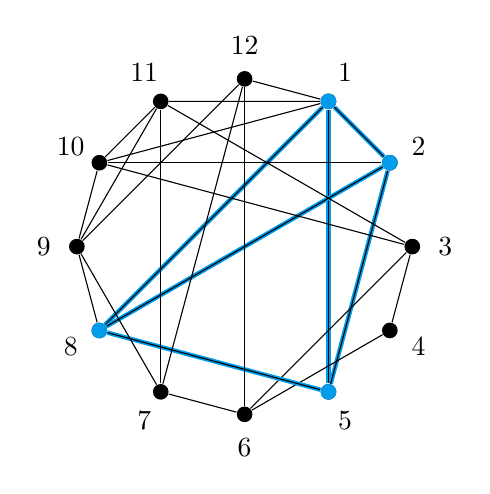
\begin{tikzpicture}
        \begin{scope}[scale=1.5]
        \newcount \myc
        \foreach \n in {3, 4, 6, 7, 9, 10, 11, 12}{
            \myc=\n \advance\myc by -1 \multiply\myc by -360 \divide\myc by 12 \advance\myc by 60
            \node[anchor=center] (L\n) at (\the\myc:1.7) {\n};
            \node[anchor=center, circle, fill=black, inner sep=2pt] (N\n) at (\the\myc:1.42) {};
        }
        \foreach \n in {1, 2, 5, 8}{
            \myc=\n \advance\myc by -1 \multiply\myc by -360 \divide\myc by 12 \advance\myc by 60
            \node[anchor=center] (L\n) at (\the\myc:1.7) {\n};
            \node<1>[anchor=center, circle, fill=black, inner sep=2pt] (N\n) at (\the\myc:1.42) {};
            \node<2>[anchor=center, circle, fill=uofgcobalt, inner sep=2pt] (N\n) at (\the\myc:1.42) {};
        }
        \draw <2> [ultra thick, color=uofgcobalt] (N1) -- (N2);
        \draw <2> [ultra thick, color=uofgcobalt] (N1) -- (N5);
        \draw <2> [ultra thick, color=uofgcobalt] (N1) -- (N8);
        \draw <1> (N1) -- (N2);
        \draw <1> (N1) -- (N5);
        \draw <1> (N1) -- (N8);
        \draw (N1) -- (N10);
        \draw (N1) -- (N11);
        \draw (N1) -- (N12);
        \draw <2> [ultra thick, color=uofgcobalt] (N2) -- (N5);
        \draw <2> [ultra thick, color=uofgcobalt] (N2) -- (N8);
        \draw <1> (N2) -- (N5);
        \draw <1> (N2) -- (N8);
        \draw (N2) -- (N10);
        \draw (N3) -- (N4);
        \draw (N3) -- (N6);
        \draw (N3) -- (N10);
        \draw (N3) -- (N11);
        \draw (N4) -- (N6);
        \draw <2> [ultra thick, color=uofgcobalt] (N5) -- (N8);
        \draw <1> (N5) -- (N8);
        \draw (N6) -- (N7);
        \draw (N6) -- (N12);
        \draw (N7) -- (N9);
        \draw (N7) -- (N11);
        \draw (N7) -- (N12);
        \draw (N8) -- (N9);
        \draw (N9) -- (N10);
        \draw (N9) -- (N11);
        \draw (N9) -- (N12);
        \draw (N10) -- (N11);
    \end{scope}
    \end{tikzpicture}
\end{center}
\end{frame}

\begin{frame}{Maximum Clique Solvers}
  There are a lot of dedicated solvers for clique problems.

    \medskip

    But there are issues:
        \begin{itemize}
            \item ``State-of-the-art'' solvers have been buggy.
            \item Often undetected: error rate of around 0.1\%.
        \end{itemize}
    \medskip
    Often used inside other solvers:
        \begin{itemize}
        \item An off-by-one result can cause much larger errors.
        \end{itemize}
\end{frame}

\begin{frame}{A Brief and Incomplete Guide to Clique Solving (1/4)}
  Recursive maximum clique algorithm:
  \begin{itemize}
  \item Pick a vertex $v$.
  \item Either $v$ is in the clique\ldots
    \begin{itemize}
    \item Throw away every vertex not adjacent to $v$.
    \item If vertices remain, recurse.
    \end{itemize}
  \item \ldots{}or $v$ is not in the clique, so
    \begin{itemize}
    \item Throw $v$ away and pick another vertex.
    \end{itemize}
  \end{itemize}
\end{frame}

\begin{frame}{A Brief and Incomplete Guide to Clique Solving (2/4)}
  Key data structures:
  \begin{itemize}
  \item Growing clique $C$.
  \item Shrinking set of potential vertices $P$.
    \begin{itemize}
    \item All the vertices we haven't thrown away yet.
    \item Every $v \in P$ is adjacent to every $w \in C$.
    \end{itemize}
  \end{itemize}
  \bigskip
  \uncover<2->{
    Branch and bound:
    \begin{itemize}
    \item Remember the biggest clique
%                     found so far, $C^\star$.
      $C^\star$ found so far.
    \item
      If
      $
      \setsize{C} + \setsize{P} \le \setsize{C^\star}
      $,
      no need to keep going.
    \end{itemize}
  }
\end{frame}

\begin{frame}{A Brief and Incomplete Guide to Clique Solving (3/4)}
  \begin{center}
    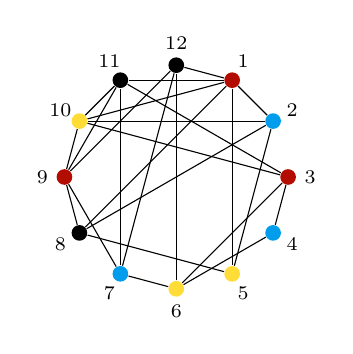
\begin{tikzpicture}
      \begin{scope}[every node/.style = {font=\scriptsize}]
        \newcount \myc
        \foreach \n in {1, 3, 9}{
          \myc=\n \advance\myc by -1 \multiply\myc by -360 \divide\myc by 12 \advance\myc by 60
          \node[anchor=center] (L\n) at (\the\myc:1.7) {\n};
          \node[anchor=center, circle, fill=uofgpillarbox, inner sep=2pt] (N\n) at (\the\myc:1.42) {};
        }
        \foreach \n in {2, 4, 7}{
          \myc=\n \advance\myc by -1 \multiply\myc by -360 \divide\myc by 12 \advance\myc by 60
          \node[anchor=center] (L\n) at (\the\myc:1.7) {\n};
          \node[anchor=center, circle, fill=uofgcobalt, inner sep=2pt] (N\n) at (\the\myc:1.42) {};
        }
        \foreach \n in {5, 6, 10}{
          \myc=\n \advance\myc by -1 \multiply\myc by -360 \divide\myc by 12 \advance\myc by 60
          \node[anchor=center] (L\n) at (\the\myc:1.7) {\n};
          \node[anchor=center, circle, fill=uofgsunshine, inner sep=2pt] (N\n) at (\the\myc:1.42) {};
        }
        \foreach \n in {8, 11, 12}{
          \myc=\n \advance\myc by -1 \multiply\myc by -360 \divide\myc by 12 \advance\myc by 60
          \node[anchor=center] (L\n) at (\the\myc:1.7) {\n};
          \node[anchor=center, circle, fill=black, inner sep=2pt] (N\n) at (\the\myc:1.42) {};
        }
        \draw (N1) -- (N2);
        \draw (N1) -- (N5);
        \draw (N1) -- (N8);
        \draw (N1) -- (N10);
        \draw (N1) -- (N11);
        \draw (N1) -- (N12);
        \draw (N2) -- (N5);
        \draw (N2) -- (N8);
        \draw (N2) -- (N10);
        \draw (N3) -- (N4);
        \draw (N3) -- (N6);
        \draw (N3) -- (N10);
        \draw (N3) -- (N11);
        \draw (N4) -- (N6);
        \draw (N5) -- (N8);
        \draw (N6) -- (N7);
        \draw (N6) -- (N12);
        \draw (N7) -- (N9);
        \draw (N7) -- (N11);
        \draw (N7) -- (N12);
        \draw (N8) -- (N9);
        \draw (N9) -- (N10);
        \draw (N9) -- (N11);
        \draw (N9) -- (N12);
        \draw (N10) -- (N11);
      \end{scope}
    \end{tikzpicture}
  \end{center}

  Given a $k$-colouring of a subgraph, that subgraph cannot have a clique of more than
  $k$ vertices.

  \medskip

  We can use $\setsize{C} + \mathit{\#colours}(P)$ as a bound, for any colouring.

\end{frame}

\begin{frame}{A Brief and Incomplete Guide to Clique Solving (4/4)}
  \begin{itemize}
  \item
    This brings us to 1997.
    \medskip
  \item
%       In practice, better bound functions, clever vertex selection
%       heuristics, efficient data structures, local search, \ldots
    Many improvements since then:
    \begin{itemize}
    \item
      better bound functions,
    \item
      clever vertex selection heuristics,
    \item
    efficient data structures,
    \item
    local search,
    \item
      \ldots
    \end{itemize}
    \medskip
  \item
    But key ideas for proof logging can be explained without worrying about such things.
  \end{itemize}
\end{frame}


\begin{frame}{Making a Proof Logging Clique Solver}
  \begin{enumerate}
  \item
    Output a pseudo-Boolean encoding of the problem.
    \begin{itemize}
    \item
      Clique problems have several standard file formats.
    \end{itemize}
    \medskip
  \item
    Make the solver log its search tree:
    \begin{itemize}
    \item
      Output a small header.
    \item
      Output something on every backtrack.
    \item
      Output something every time a solution is found.
    \item
      Output a small footer.
    \end{itemize}
    \medskip
  \item
    Figure out how to log the bound function.
  \end{enumerate}
\end{frame}

\begin{frame}{A Slightly Different Workflow}
    \begin{center}
        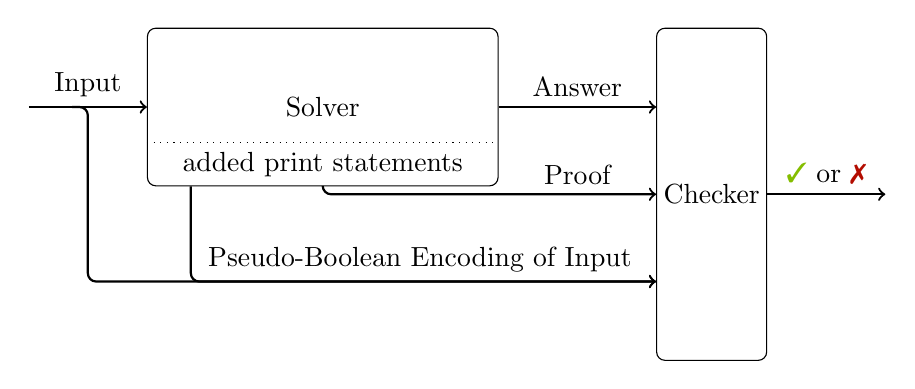
\begin{tikzpicture}
            \node (solver) [inner xsep=5em, inner ysep=2.5em, draw, rounded corners=3pt] { Solver };

            \node (checker) [right=2cm of solver.north east, anchor=north west,
            inner xsep=0.25em, draw, rounded corners=3pt, minimum height=12em, visible on=<3->] { Checker };

            \node (print) [anchor=south, above=0cm of solver.south, visible on=<2->] { added print statements };
            \draw [dotted, visible on=<2->] (solver.west|-print.north) -- (solver.east|-print.north);

            \draw [->, thick] (solver.east) -- (solver.east -| checker.west)
                coordinate [midway] (solutionmid) node [above, midway] { Answer };

            \draw [->, thick, rounded corners=3pt, visible on=<2->] (solver.south) -- (solver.south |- checker.west)
                -- (checker.west) coordinate [midway] (proofmid);

            \coordinate (prooflabel) at (proofmid-|solutionmid);
            \node [above=0cm of prooflabel, visible on=<2->] { Proof };

            \coordinate [right=1.5cm of checker.east] (verified);
            \draw [->, thick, visible on=<5->] (checker.east) -- (verified) node [above, midway] { \textcolor{uofglawn}{\ding{51}} or \textcolor{uofgpillarbox}{\ding{55}} };

            \coordinate [left=1.5cm of solver.west] (input);
            \draw [->, thick] (input) -- (solver.west) coordinate [midway] (inputmid) node [above, midway] { Input };

            \coordinate (checkerbotleft) at ($(checker.west)+($(checker.west)-(solver.east-|checker.west)$)$);

            \draw [->, thick, rounded corners=3pt, visible on=<3>] ($(inputmid)+(-0.2,0)$) --
            (inputmid) -- (inputmid |- checkerbotleft) -- (checkerbotleft) coordinate [midway] (altinputmid);
            \coordinate (solverstart) at ($(solver.south)!0.75!(solver.south west)$);
            \draw [->, thick, rounded corners=3pt, visible on=<4->] (solverstart) -- (solverstart |- checkerbotleft) -- (checkerbotleft);

            \coordinate (encinputlabel) at (altinputmid-|solutionmid);
            \node [above=0cm of encinputlabel, xshift=-2cm, visible on=<4->] { Pseudo-Boolean Encoding of Input };
        \end{tikzpicture}
    \end{center}
\end{frame}

\begin{frame}[fragile]{A Pseudo-Boolean Encoding for Clique (in OPB Format)}
    \begin{center}
    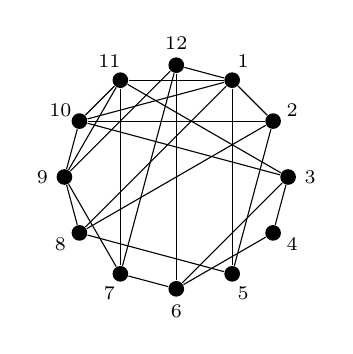
\begin{tikzpicture}
        \begin{scope}[every node/.style = {font=\scriptsize}]
        \newcount \myc
        \foreach \n in {3, 4, 6, 7, 9, 10, 11, 12}{
            \myc=\n \advance\myc by -1 \multiply\myc by -360 \divide\myc by 12 \advance\myc by 60
            \node[anchor=center] (L\n) at (\the\myc:1.7) {\n};
            \node[anchor=center, circle, fill=black, inner sep=2pt] (N\n) at (\the\myc:1.42) {};
        }
        \foreach \n in {1, 2, 5, 8}{
            \myc=\n \advance\myc by -1 \multiply\myc by -360 \divide\myc by 12 \advance\myc by 60
            \node[anchor=center] (L\n) at (\the\myc:1.7) {\n};
            \node[anchor=center, circle, fill=black, inner sep=2pt] (N\n) at (\the\myc:1.42) {};
        }
            \draw  (N1) -- (N2);
            \draw  (N1) -- (N5);
            \draw  (N1) -- (N8);
        \draw (N1) -- (N10);
        \draw (N1) -- (N11);
        \draw (N1) -- (N12);
            \draw  (N2) -- (N5);
            \draw  (N2) -- (N8);
        \draw (N2) -- (N10);
        \draw (N3) -- (N4);
        \draw (N3) -- (N6);
        \draw (N3) -- (N10);
        \draw (N3) -- (N11);
        \draw (N4) -- (N6);
            \draw  (N5) -- (N8);
        \draw (N6) -- (N7);
        \draw (N6) -- (N12);
        \draw (N7) -- (N9);
        \draw (N7) -- (N11);
        \draw (N7) -- (N12);
        \draw (N8) -- (N9);
        \draw (N9) -- (N10);
        \draw (N9) -- (N11);
        \draw (N9) -- (N12);
        \draw (N10) -- (N11);
    \end{scope}
    \end{tikzpicture}
\end{center}

\small\begin{Verbatim}[commandchars=\\\{\},codes={\catcode`$=3\catcode`^=7}]
\colorblue{* #variable= 12 #constraint= 41}
min: -1 x1 -1 x2 -1 x3 -1 x4 \emph{\ldots{}and so on\ldots{}} -1 x11 -1 x12 ;
1 ~x3 1 ~x1 >= 1 ;
1 ~x3 1 ~x2 >= 1 ;
1 ~x4 1 ~x1 >= 1 ;
\colorblue{* \ldots{}and a further 38 similar lines for the remaining non-edges}
\end{Verbatim}
\end{frame}

\begin{frame}[fragile,t]{First Attempt at a Proof}%
\only<2>{
\begin{tikzpicture}[overlay,remember picture] \coordinate (cliqueheader1space) at ($(pic cs:cliqueheader1)+(0pt,6pt)$); \node[rounded corners, fit = (cliqueheader1space) (pic cs:cliqueheader2) (pic cs:cliqueheader3), fill=uofgsunshine] {};\end{tikzpicture}}%
\only<6>{
\begin{tikzpicture}[overlay,remember picture] \coordinate (opt1space) at ($(pic cs:opt1a)+(0pt,6pt)$); \node[rounded corners, fit = (opt1space) (pic cs:opt1b), fill=uofgsunshine] {};\end{tikzpicture}}%
\only<7>{
\begin{tikzpicture}[overlay,remember picture] \coordinate (bt1space) at ($(pic cs:bt1a)+(0pt,6pt)$); \node[rounded corners, fit = (bt1space) (pic cs:bt1b), fill=uofgsunshine] {};\end{tikzpicture}}%
\only<8>{
\begin{tikzpicture}[overlay,remember picture] \coordinate (bt2space) at ($(pic cs:bt2a)+(0pt,6pt)$); \node[rounded corners, fit = (bt2space) (pic cs:bt2b), fill=uofgsunshine] {};\end{tikzpicture}}%
\only<9>{
\begin{tikzpicture}[overlay,remember picture] \coordinate (bt3space) at ($(pic cs:bt3a)+(0pt,6pt)$); \node[rounded corners, fit = (bt3space) (pic cs:bt3b), fill=uofgsunshine] {};\end{tikzpicture}}%
\only<10>{
\begin{tikzpicture}[overlay,remember picture] \coordinate (bt4space) at ($(pic cs:bt4a)+(0pt,6pt)$); \node[rounded corners, fit = (bt4space) (pic cs:bt4b), fill=uofgsunshine] {};\end{tikzpicture}}%
\only<11>{
\begin{tikzpicture}[overlay,remember picture] \coordinate (opt2space) at ($(pic cs:opt2a)+(0pt,6pt)$); \node[rounded corners, fit = (opt2space) (pic cs:opt2b), fill=uofgsunshine] {};\end{tikzpicture}}%
\only<12>{
\begin{tikzpicture}[overlay,remember picture] \coordinate (bt5space) at ($(pic cs:bt5a)+(0pt,6pt)$); \node[rounded corners, fit = (bt5space) (pic cs:bt5b), fill=uofgsunshine] {};\end{tikzpicture}}%
\only<13>{
\begin{tikzpicture}[overlay,remember picture] \coordinate (bt6space) at ($(pic cs:bt6a)+(0pt,6pt)$); \node[rounded corners, fit = (bt6space) (pic cs:bt6b), fill=uofgsunshine] {};\end{tikzpicture}}%
\only<14>{
\begin{tikzpicture}[overlay,remember picture] \coordinate (bt7space) at ($(pic cs:bt7a)+(0pt,6pt)$); \node[rounded corners, fit = (bt7space) (pic cs:bt7b), fill=uofgsunshine] {};\end{tikzpicture}}%
\only<15>{
\begin{tikzpicture}[overlay,remember picture] \coordinate (contaspace) at ($(pic cs:conta)+(0pt,6pt)$); \node[rounded corners, fit = (contaspace) (pic cs:contb), fill=uofgsunshine] {};\end{tikzpicture}}%
\begin{tikzpicture}[overlay,remember picture]
    \node [xshift=-3cm, yshift=0.5cm] at (current page.east) {
        \begin{tikzpicture}
    \begin{scope}[every node/.style = {font=\scriptsize}]

        \myc=1 \advance\myc by -1 \multiply\myc by -360 \divide\myc by 12 \advance\myc by 60
        \node[anchor=center] (L1) at (\the\myc:1.7) {1};
        \node<1-3>[anchor=center, circle, fill=black, inner sep=2pt] (N1) at (\the\myc:1.42) {};
        \node<4-6>[anchor=center, circle, fill=black!20, inner sep=2pt] (N1) at (\the\myc:1.42) {};
        \node<7>[anchor=center, circle, fill=black!20, inner sep=2pt] (N1) at (\the\myc:1.42) {};
        \node<8>[anchor=center, circle, fill=black, inner sep=2pt] (N1) at (\the\myc:1.42) {};
        \node<9-10>[anchor=center, circle, fill=black, inner sep=2pt] (N1) at (\the\myc:1.42) {};
        \node<11>[anchor=center, circle, fill=uofgcobalt, inner sep=2pt] (N1) at (\the\myc:1.42) {};
        \node<12->[anchor=center, circle, fill=black, inner sep=2pt] (N1) at (\the\myc:1.42) {};

        \myc=2 \advance\myc by -1 \multiply\myc by -360 \divide\myc by 12 \advance\myc by 60
        \node[anchor=center] (L2) at (\the\myc:1.7) {2};
        \node<1-2>[anchor=center, circle, fill=black, inner sep=2pt] (N2) at (\the\myc:1.42) {};
        \node<3-10>[anchor=center, circle, fill=black!20, inner sep=2pt] (N2) at (\the\myc:1.42) {};
        \node<11>[anchor=center, circle, fill=uofgcobalt, inner sep=2pt] (N2) at (\the\myc:1.42) {};
        \node<12->[anchor=center, circle, fill=black, inner sep=2pt] (N2) at (\the\myc:1.42) {};

        \myc=3 \advance\myc by -1 \multiply\myc by -360 \divide\myc by 12 \advance\myc by 60
        \node[anchor=center] (L3) at (\the\myc:1.7) {3};
        \node<1-2>[anchor=center, circle, fill=black, inner sep=2pt] (N3) at (\the\myc:1.42) {};
        \node<3-6>[anchor=center, circle, fill=black!20, inner sep=2pt] (N3) at (\the\myc:1.42) {};
        \node<7>[anchor=center, circle, fill=black!20, inner sep=2pt] (N3) at (\the\myc:1.42) {};
        \node<8>[anchor=center, circle, fill=black!20, inner sep=2pt] (N3) at (\the\myc:1.42) {};
        \node<9-10>[anchor=center, circle, fill=black, inner sep=2pt] (N3) at (\the\myc:1.42) {};
        \node<11-13>[anchor=center, circle, fill=black!20, inner sep=2pt] (N3) at (\the\myc:1.42) {};
        \node<14->[anchor=center, circle, fill=black, inner sep=2pt] (N3) at (\the\myc:1.42) {};

        \myc=4 \advance\myc by -1 \multiply\myc by -360 \divide\myc by 12 \advance\myc by 60
        \node[anchor=center] (L4) at (\the\myc:1.7) {4};
        \node<1-2>[anchor=center, circle, fill=black, inner sep=2pt] (N4) at (\the\myc:1.42) {};
        \node<3-13>[anchor=center, circle, fill=black!20, inner sep=2pt] (N4) at (\the\myc:1.42) {};
        \node<14->[anchor=center, circle, fill=black, inner sep=2pt] (N4) at (\the\myc:1.42) {};

        \myc=5 \advance\myc by -1 \multiply\myc by -360 \divide\myc by 12 \advance\myc by 60
        \node[anchor=center] (L5) at (\the\myc:1.7) {5};
        \node<1-2>[anchor=center, circle, fill=black, inner sep=2pt] (N5) at (\the\myc:1.42) {};
        \node<3-10>[anchor=center, circle, fill=black!20, inner sep=2pt] (N5) at (\the\myc:1.42) {};
        \node<11>[anchor=center, circle, fill=uofgcobalt, inner sep=2pt] (N5) at (\the\myc:1.42) {};
        \node<12>[anchor=center, circle, fill=uofgthistle, inner sep=2pt] (N5) at (\the\myc:1.42) {};
        \node<13>[anchor=center, circle, fill=black!20, inner sep=2pt] (N5) at (\the\myc:1.42) {};
        \node<14->[anchor=center, circle, fill=black, inner sep=2pt] (N5) at (\the\myc:1.42) {};

        \myc=6 \advance\myc by -1 \multiply\myc by -360 \divide\myc by 12 \advance\myc by 60
        \node[anchor=center] (L6) at (\the\myc:1.7) {6};
        \node<1-4>[anchor=center, circle, fill=black, inner sep=2pt] (N6) at (\the\myc:1.42) {};
        \node<5-6>[anchor=center, circle, fill=black!20, inner sep=2pt] (N6) at (\the\myc:1.42) {};
        \node<7-8>[anchor=center, circle, fill=black, inner sep=2pt] (N6) at (\the\myc:1.42) {};
        \node<9-13>[anchor=center, circle, fill=black!20, inner sep=2pt] (N6) at (\the\myc:1.42) {};
        \node<14->[anchor=center, circle, fill=black, inner sep=2pt] (N6) at (\the\myc:1.42) {};

        \myc=7 \advance\myc by -1 \multiply\myc by -360 \divide\myc by 12 \advance\myc by 60
        \node[anchor=center] (L7) at (\the\myc:1.7) {7};
        \node<1-3>[anchor=center, circle, fill=black, inner sep=2pt] (N7) at (\the\myc:1.42) {};
        \node<4-6>[anchor=center, circle, fill=uofgcobalt, inner sep=2pt] (N7) at (\the\myc:1.42) {};
        \node<7>[anchor=center, circle, fill=uofgthistle, inner sep=2pt] (N7) at (\the\myc:1.42) {};
        \node<8-9>[anchor=center, circle, fill=black!20, inner sep=2pt] (N7) at (\the\myc:1.42) {};
        \node<10>[anchor=center, circle, fill=black, inner sep=2pt] (N7) at (\the\myc:1.42) {};
        \node<11-13>[anchor=center, circle, fill=black!20, inner sep=2pt] (N7) at (\the\myc:1.42) {};
        \node<14->[anchor=center, circle, fill=black, inner sep=2pt] (N7) at (\the\myc:1.42) {};

        \myc=8 \advance\myc by -1 \multiply\myc by -360 \divide\myc by 12 \advance\myc by 60
        \node<1-13>[anchor=center] (L8) at (\the\myc:1.7) {8};
        \node<14->[anchor=center] (L8) at (\the\myc:1.7) {\phantom{8}};
        \node<1-2>[anchor=center, circle, fill=black, inner sep=2pt] (N8) at (\the\myc:1.42) {};
        \node<3-10>[anchor=center, circle, fill=black!20, inner sep=2pt] (N8) at (\the\myc:1.42) {};
        \node<11>[anchor=center, circle, fill=uofgcobalt, inner sep=2pt] (N8) at (\the\myc:1.42) {};
        \node<12-13>[anchor=center, circle, fill=uofgthistle, inner sep=2pt] (N8) at (\the\myc:1.42) {};

        \myc=9 \advance\myc by -1 \multiply\myc by -360 \divide\myc by 12 \advance\myc by 60
        \node[anchor=center] (L9) at (\the\myc:1.7) {9};
        \node<1-4>[anchor=center, circle, fill=black, inner sep=2pt] (N9) at (\the\myc:1.42) {};
        \node<5-6>[anchor=center, circle, fill=uofgcobalt, inner sep=2pt] (N9) at (\the\myc:1.42) {};
        \node<7>[anchor=center, circle, fill=black, inner sep=2pt] (N9) at (\the\myc:1.42) {};
        \node<8>[anchor=center, circle, fill=black, inner sep=2pt] (N9) at (\the\myc:1.42) {};
        \node<9-10>[anchor=center, circle, fill=black, inner sep=2pt] (N9) at (\the\myc:1.42) {};
        \node<11-12>[anchor=center, circle, fill=black!20, inner sep=2pt] (N9) at (\the\myc:1.42) {};
        \node<13->[anchor=center, circle, fill=black, inner sep=2pt] (N9) at (\the\myc:1.42) {};

        \myc=10 \advance\myc by -1 \multiply\myc by -360 \divide\myc by 12 \advance\myc by 60
        \node[anchor=center] (L10) at (\the\myc:1.7) {10};
        \node<1-2>[anchor=center, circle, fill=black, inner sep=2pt] (N10) at (\the\myc:1.42) {};
        \node<3-6>[anchor=center, circle, fill=black!20, inner sep=2pt] (N10) at (\the\myc:1.42) {};
        \node<7>[anchor=center, circle, fill=black!20, inner sep=2pt] (N10) at (\the\myc:1.42) {};
        \node<8>[anchor=center, circle, fill=black!20, inner sep=2pt] (N10) at (\the\myc:1.42) {};
        \node<9>[anchor=center, circle, fill=uofgthistle, inner sep=2pt] (N10) at (\the\myc:1.42) {};
        \node<10-13>[anchor=center, circle, fill=black!20, inner sep=2pt] (N10) at (\the\myc:1.42) {};
        \node<14->[anchor=center, circle, fill=black, inner sep=2pt] (N10) at (\the\myc:1.42) {};

        \myc=11 \advance\myc by -1 \multiply\myc by -360 \divide\myc by 12 \advance\myc by 60
        \node<1-10>[anchor=center] (L11) at (\the\myc:1.7) {11};
        \node<11->[anchor=center] (L11) at (\the\myc:1.7) {\phantom{11}};
        \node<1-2>[anchor=center, circle, fill=black, inner sep=2pt] (N11) at (\the\myc:1.42) {};
        \node<3-6>[anchor=center, circle, fill=black!20, inner sep=2pt] (N11) at (\the\myc:1.42) {};
        \node<7>[anchor=center, circle, fill=black!20, inner sep=2pt] (N11) at (\the\myc:1.42) {};
        \node<8>[anchor=center, circle, fill=black!20, inner sep=2pt] (N11) at (\the\myc:1.42) {};
        \node<9-10>[anchor=center, circle, fill=uofgthistle, inner sep=2pt] (N11) at (\the\myc:1.42) {};

        \myc=12 \advance\myc by -1 \multiply\myc by -360 \divide\myc by 12 \advance\myc by 60
        \node<1-8>[anchor=center] (L12) at (\the\myc:1.7) {12};
        \node<9->[anchor=center] (L12) at (\the\myc:1.7) {\phantom{12}};
        \node<1-2>[anchor=center, circle, fill=black, inner sep=2pt] (N12) at (\the\myc:1.42) {};
        \node<3-6>[anchor=center, circle, fill=uofgcobalt, inner sep=2pt] (N12) at (\the\myc:1.42) {};
        \node<7-8>[anchor=center, circle, fill=uofgthistle, inner sep=2pt] (N12) at (\the\myc:1.42) {};

        \draw <1-2> (N1) -- (N2);
        \draw <3-10> [color=black!20] (N1) -- (N2);
        \draw <11> [ultra thick, color=uofgcobalt] (N1) -- (N2);
        \draw <12-> (N1) -- (N2);

        \draw <1-2> (N1) -- (N5);
        \draw <3-10> [color=black!20] (N1) -- (N5);
        \draw <11> [ultra thick, color=uofgcobalt] (N1) -- (N5);
        \draw <12> (N1) -- (N5);
        \draw <13> [color=black!20] (N1) -- (N5);
        \draw <14-> (N1) -- (N5);

        \draw <1-2> (N1) -- (N8);
        \draw <3-10> [color=black!20] (N1) -- (N8);
        \draw <11> [ultra thick, color=uofgcobalt] (N1) -- (N8);
        \draw <12-13> (N1) -- (N8);

        \draw <1-2> (N1) -- (N10);
        \draw <3-8> [color=black!20] (N1) -- (N10);
        \draw <9> (N1) -- (N10);
        \draw <10-13> [color=black!20] (N1) -- (N10);
        \draw <14-> (N1) -- (N10);

        \draw <1-2> (N1) -- (N11);
        \draw <3-8> [color=black!20] (N1) -- (N11);
        \draw <9-10> (N1) -- (N11);

        \draw <1-3> (N1) -- (N12);
        \draw <4-7> [color=black!20] (N1) -- (N12);
        \draw <8> (N1) -- (N12);

        \draw <1-2> (N2) -- (N5);
        \draw <3-10> [color=black!20] (N2) -- (N5);
        \draw <11> [ultra thick, color=uofgcobalt] (N2) -- (N5);
        \draw <12> (N2) -- (N5);
        \draw <13> [color=black!20] (N2) -- (N5);
        \draw <14-> (N2) -- (N5);

        \draw <1-2> (N2) -- (N8);
        \draw <3-10> [color=black!20] (N2) -- (N8);
        \draw <11> [ultra thick, color=uofgcobalt](N2) -- (N8);
        \draw <12-13> (N2) -- (N8);

        \draw <1-2> (N2) -- (N10);
        \draw <3-13> [color=black!20] (N2) -- (N10);
        \draw <14-> (N2) -- (N10);

        \draw <1-2> (N3) -- (N4);
        \draw <3-13> [color=black!20] (N3) -- (N4);
        \draw <14-> (N3) -- (N4);

        \draw <1-2> (N3) -- (N6);
        \draw <3-13> [color=black!20] (N3) -- (N6);
        \draw <14-> (N3) -- (N6);

        \draw <1-2> (N3) -- (N10);
        \draw <3-8> [color=black!20] (N3) -- (N10);
        \draw <9> (N3) -- (N10);
        \draw <10-13> [color=black!20] (N3) -- (N10);
        \draw <14-> (N3) -- (N10);

        \draw <1-2> (N3) -- (N11);
        \draw <3-8> [color=black!20] (N3) -- (N11);
        \draw <9-10> (N3) -- (N11);

        \draw <1-2> (N4) -- (N6);
        \draw <3-13> [color=black!20] (N4) -- (N6);
        \draw <14-> (N4) -- (N6);

        \draw <1-2> (N5) -- (N8);
        \draw <3-10> [color=black!20] (N5) -- (N8);
        \draw <11> [ultra thick, color=uofgcobalt] (N5) -- (N8);
        \draw <12> [ultra thick, color=uofgthistle] (N5) -- (N8);

        \draw <1-4> (N6) -- (N7);
        \draw <5-6> [color=black!20] (N6) -- (N7);
        \draw <7> (N6) -- (N7);
        \draw <8-13> [color=black!20] (N6) -- (N7);
        \draw <14-> (N6) -- (N7);

        \draw <1-4> (N6) -- (N12);
        \draw <5-6> [color=black!20] (N6) -- (N12);
        \draw <7-8> (N6) -- (N12);

        \draw <1-5> (N7) -- (N9);
        \draw <6> [ultra thick, color=uofgcobalt] (N7) -- (N9);
        \draw <7> (N7) -- (N9);
        \draw <8-9> [color=black!20] (N7) -- (N9);
        \draw <10> (N7) -- (N9);
        \draw <11-13> [color=black!20] (N7) -- (N9);
        \draw <14-> (N7) -- (N9);

        \draw <1-2> (N7) -- (N11);
        \draw <3-9> [color=black!20] (N7) -- (N11);
        \draw <10> (N7) -- (N11);

        \draw <1-5> (N7) -- (N12);
        \draw <6> [ultra thick, color=uofgcobalt] (N7) -- (N12);
        \draw <7> [ultra thick, color=uofgthistle] (N7) -- (N12);

        \draw <1-2> (N8) -- (N9);
        \draw <3-12> [color=black!20] (N8) -- (N9);
        \draw <13> (N8) -- (N9);

        \draw <1-2> (N9) -- (N10);
        \draw <3-8> [color=black!20] (N9) -- (N10);
        \draw <9> (N9) -- (N10);
        \draw <10-13> [color=black!20] (N9) -- (N10);
        \draw <14-> (N9) -- (N10);

        \draw <1-2> (N9) -- (N11);
        \draw <3-8> [color=black!20] (N9) -- (N11);
        \draw <9-10> (N9) -- (N11);

        \draw <1-5> (N9) -- (N12);
        \draw <6> [ultra thick, color=uofgcobalt] (N9) -- (N12);
        \draw <7-8> (N9) -- (N12);

        \draw <1-2> (N10) -- (N11);
        \draw <3-8> [color=black!20] (N10) -- (N11);
        \draw <9> [ultra thick, color=uofgthistle] (N10) -- (N11);
\end{scope}
        \end{tikzpicture}};\end{tikzpicture}%
\begin{tikzpicture}[overlay,remember picture]
    \node <2-> [anchor=south east, text depth=1.5cm, rounded corners=3pt, fill=uofgsunshine, draw, yshift=0.9cm, xshift=-0.5cm]
    at (current page.south east) {
        \begin{minipage}[t]{0.5\paperwidth}\raggedright
        \only<2>{Start with a header\\Load the 41 problem axioms}%
            \only<3>{Branch accepting $12$ \\Throw away non-adjacent vertices}%
            \only<4>{Branch also accepting $7$ \\Throw away non-adjacent vertices}%
            \only<5>{Branch also accepting $9$ \\Throw away non-adjacent vertices}%
        \only<6>{We branched on $12$, $7$, $9$\\Found a new incumbent\\Now looking for a $\ge 4$ vertex clique}%
            \only<7>{Backtrack from $12$, $7$\\$9$ explored already, only $6$ feasible\\No $\ge 4$ vertex clique possible\\Effectively this deletes the $7$--$12$ edge}%
            \only<8>{Backtrack from $12$\\Only $1$, $6$ and $9$ feasible (1-colourable)\\No $\ge 4$ vertex clique possible\\Effectively this deletes vertex $12$}%
            \only<9>{Branch on $11$ then $10$\\Only $1$, $3$ and $9$ feasible (1-colourable)\\No $\ge 4$ vertex clique possible\\Backtrack, deleting the edge}%
        \only<10>{Backtrack from $11$\\2-colourable, so no $\ge 4$ clique\\Delete the vertex}%
        \only<11>{Branch on $8$, $5$, $1$, $2$\\Find a new incumbent\\Now looking for a $\ge 5$ vertex clique}%
        \only<12>{Backtrack from $8$, $5$\\Only 4 vertices; can't have a $\ge 5$ clique\\Delete the edge}%
        \only<13>{Backtrack from $8$\\Still not enough vertices\\Delete the vertex}%
        \only<14>{%
          %%% Just experimenting, Ciaran --- feel free to change back -JN
%             Now obvious to a solver that we can't find a $5$-clique anywhere
%             (we'll see why)%
            Remaining graph is 3-colourable\\Backtrack from root node}%
        \only<15>{%
          %%% Just experimenting, Ciaran --- feel free to change back -JN
            Finish with what we've concluded\\
            We specify a lower and an upper bound\\
            Remember we're minimising $\sum_v -1 \times v$, so a $4$-clique has an
            objective value of $-4$\\
        }%
        \end{minipage}
    };
\end{tikzpicture}
\vspace*{-0.5cm}\begin{Verbatim}[commandchars=\\\{\},codes={\catcode`$=3\catcode`^=7}]
\tikzmark{cliqueheader1}pseudo-Boolean proof version 2.0\tikzmark{cliqueheader2}
f 41\tikzmark{cliqueheader3}
\tikzmark{opt1a}soli x7 x9 x12\tikzmark{opt1b}
\tikzmark{bt1a}rup 1 ~x12 1 ~x7 >= 1 ;\tikzmark{bt1b}
\tikzmark{bt2a}rup 1 ~x12 >= 1 ;\tikzmark{bt2b}
\tikzmark{bt3a}rup 1 ~x11 1 ~x10 >= 1 ;\tikzmark{bt3b}
\tikzmark{bt4a}rup 1 ~x11 >= 1 ;\tikzmark{bt4b}
\tikzmark{opt2a}soli x1 x2 x5 x8\tikzmark{opt2b}
\tikzmark{bt5a}rup 1 ~x8 1 ~x5 >= 1 ;\tikzmark{bt5b}
\tikzmark{bt6a}rup 1 ~x8 >= 1 ;\tikzmark{bt6b}
\tikzmark{bt7a}rup >= 1 ;\tikzmark{bt7b}
\tikzmark{conta}output NONE
conclusion BOUNDS -4 -4
end pseudo-Boolean proof\tikzmark{contb}
\end{Verbatim}
\end{frame}

\begin{frame}[fragile,t]{Verifying This Proof (Or Not\ldots)}
\begin{onlyenv}<1-2>\footnotesize
\begin{Verbatim}
$ veripb clique.opb clique-attempt-one.veripb
Verification failed.
Failed in proof file line 6.
Hint: Failed to show '1 ~x10 1 ~x11 >= 1' by reverse unit propagation.
\end{Verbatim}

    \begin{center}\only<2>{
        \begin{tikzpicture}
    \begin{scope}[every node/.style = {font=\scriptsize}]

        \myc=1 \advance\myc by -1 \multiply\myc by -360 \divide\myc by 12 \advance\myc by 60
        \node[anchor=center] (L1) at (\the\myc:1.7) {1};
        \node[anchor=center, circle, fill=black, inner sep=2pt] (N1) at (\the\myc:1.42) {};

        \myc=2 \advance\myc by -1 \multiply\myc by -360 \divide\myc by 12 \advance\myc by 60
        \node[anchor=center] (L2) at (\the\myc:1.7) {2};
        \node[anchor=center, circle, fill=black!20, inner sep=2pt] (N2) at (\the\myc:1.42) {};

        \myc=3 \advance\myc by -1 \multiply\myc by -360 \divide\myc by 12 \advance\myc by 60
        \node[anchor=center] (L3) at (\the\myc:1.7) {3};
        \node[anchor=center, circle, fill=black, inner sep=2pt] (N3) at (\the\myc:1.42) {};

        \myc=4 \advance\myc by -1 \multiply\myc by -360 \divide\myc by 12 \advance\myc by 60
        \node[anchor=center] (L4) at (\the\myc:1.7) {4};
        \node[anchor=center, circle, fill=black!20, inner sep=2pt] (N4) at (\the\myc:1.42) {};

        \myc=5 \advance\myc by -1 \multiply\myc by -360 \divide\myc by 12 \advance\myc by 60
        \node[anchor=center] (L5) at (\the\myc:1.7) {5};
        \node[anchor=center, circle, fill=black!20, inner sep=2pt] (N5) at (\the\myc:1.42) {};

        \myc=6 \advance\myc by -1 \multiply\myc by -360 \divide\myc by 12 \advance\myc by 60
        \node[anchor=center] (L6) at (\the\myc:1.7) {6};
        \node[anchor=center, circle, fill=black!20, inner sep=2pt] (N6) at (\the\myc:1.42) {};

        \myc=7 \advance\myc by -1 \multiply\myc by -360 \divide\myc by 12 \advance\myc by 60
        \node[anchor=center] (L7) at (\the\myc:1.7) {7};
        \node[anchor=center, circle, fill=black!20, inner sep=2pt] (N7) at (\the\myc:1.42) {};

        \myc=8 \advance\myc by -1 \multiply\myc by -360 \divide\myc by 12 \advance\myc by 60
        \node[anchor=center] (L8) at (\the\myc:1.7) {8};
        \node[anchor=center, circle, fill=black!20, inner sep=2pt] (N8) at (\the\myc:1.42) {};

        \myc=9 \advance\myc by -1 \multiply\myc by -360 \divide\myc by 12 \advance\myc by 60
        \node[anchor=center] (L9) at (\the\myc:1.7) {9};
        \node[anchor=center, circle, fill=black, inner sep=2pt] (N9) at (\the\myc:1.42) {};

        \myc=10 \advance\myc by -1 \multiply\myc by -360 \divide\myc by 12 \advance\myc by 60
        \node[anchor=center] (L10) at (\the\myc:1.7) {10};
        \node[anchor=center, circle, fill=uofgthistle, inner sep=2pt] (N10) at (\the\myc:1.42) {};

        \myc=11 \advance\myc by -1 \multiply\myc by -360 \divide\myc by 12 \advance\myc by 60
        \node[anchor=center] (L11) at (\the\myc:1.7) {11};
        \node[anchor=center, circle, fill=uofgthistle, inner sep=2pt] (N11) at (\the\myc:1.42) {};

        \myc=12 \advance\myc by -1 \multiply\myc by -360 \divide\myc by 12 \advance\myc by 60
        \node[anchor=center] (L12) at (\the\myc:1.7) {\phantom{12}};

        \draw [color=black!20] (N1) -- (N2);
        \draw [color=black!20] (N1) -- (N5);
        \draw [color=black!20] (N1) -- (N8);
        \draw (N1) -- (N10);
        \draw (N1) -- (N11);
        \draw [color=black!20] (N2) -- (N5);
        \draw [color=black!20] (N2) -- (N8);
        \draw [color=black!20] (N2) -- (N10);
        \draw [color=black!20] (N3) -- (N4);
        \draw [color=black!20] (N3) -- (N6);
        \draw (N3) -- (N10);
        \draw (N3) -- (N11);
        \draw [color=black!20] (N5) -- (N8);
        \draw [color=black!20] (N6) -- (N7);
        \draw [color=black!20] (N7) -- (N9);
        \draw [color=black!20] (N7) -- (N11);
        \draw [color=black!20] (N8) -- (N9);
        \draw (N9) -- (N10);
        \draw (N9) -- (N11);
        \draw [ultra thick, color=uofgthistle] (N10) -- (N11);
    \end{scope}\end{tikzpicture}}\end{center}
\end{onlyenv}\begin{onlyenv}<3>%
\begin{Verbatim}[commandchars=\\\{\}]
$ veripb --trace clique.opb clique-attempt-one.veripb
line 002: f 41
  ConstraintId \veripbid{001}: \veripbConstraint{1 ~x1 1 ~x3 >= 1}
  ConstraintId \veripbid{002}: \veripbConstraint{1 ~x2 1 ~x3 >= 1}
...
  ConstraintId \veripbid{041}: \veripbConstraint{1 ~x11 1 ~x12 >= 1}
line 003: soli x7 x9 x12 ~x1 ~x2 ~x3 ~x4 ~x5 ~x6 ~x8 ~x10 ~x11
  ConstraintId \veripbid{042}: \veripbConstraint{1 x1 1 x2 1 x3 1 x4 1 x5 1 x6 1 x7 1 x8 1 x9 1 x10 1 x11 1 x12 >= 4}
line 004: rup 1 ~x12 1 ~x7 >= 1 ;
  ConstraintId \veripbid{043}: \veripbConstraint{1 ~x7 1 ~x12 >= 1}
line 005: rup 1 ~x12 >= 1 ;
  ConstraintId \veripbid{044}: \veripbConstraint{1 ~x12 >= 1}
line 006: rup 1 ~x11 1 ~x10 >= 1 ;
Verification failed.
Failed in proof file line 6.
Hint: Failed to show '1 ~x10 1 ~x11 >= 1' by reverse unit propagation.
\end{Verbatim}
\end{onlyenv}
\end{frame}

\begin{frame}{Dealing With Colourings}

  \vspace{-1mm}

    The colour bound doesn't follow by RUP\ldots

    \medskip

%       We
    But we
    can lazily recover at-most-one constraints for each colour class!
    \uncover<2->{
      \begin{align*}
        (\overline{x}_1 + \overline{x}_6 \ge 1)
% \,\times\,2
&
%    &=~&
%   2\overline{x}_1 + 2\overline{x}_6 \ge 2
\\
        +\,(\overline{x}_1 + \overline{x}_9 \ge 1) & &=~&
2 \overline{x}_1 +
\hphantom{2} \overline{x}_6 +
\hphantom{2} \overline{x}_9
\ge 2 \\
        +\,(\overline{x}_6 + \overline{x}_9 \ge 1) & &=~&
2 \overline{x}_1 +
2 \overline{x}_6 +
2 \overline{x}_9
\ge 3 \\
%           /\,3
        /\,2
& &=~&
\hphantom{2} \overline{x}_1 +
\hphantom{2} \overline{x}_6 +
\hphantom{2} \overline{x}_9
\ge 2 \\
 && \text{i.e.}~ & x_1 + x_6 + x_9 \le 1
    \end{align*}}
  \uncover<3->{
    This generalises
%    for arbitrarily large colour classes
    to colour classes of any size~$v$.
    \begin{itemize}
        \item
          Each non-edge is used exactly once, $v (v - 1)$ additions
        \item
%             $v - 2$ multiplications and divisions
          $v - 3$ multiplications and $v-2$ divisions.
    \end{itemize}
    Solvers don't need to ``understand'' cutting planes to
%   write this out
    write this derivation to proof log.
  }
\end{frame}

\newcommand{\notedge}{\not\sim}

\begin{nearlyplainframe}[t]{What This Looks Like
    in the Proof Log
}

\vspace{-1.5mm}

\begin{minipage}[t]{0.45\framewidth}
\VerbatimInput[commandchars=\\\{\},codes={\catcode`$=3\catcode`^=7\catcode`_=8}]{clique-proof-1.veripb}
\end{minipage}\hfill\begin{minipage}[t]{0.45\framewidth}
\VerbatimInput[commandchars=\\\{\},codes={\catcode`$=3\catcode`^=7\catcode`_=8}]{clique-proof-2.veripb}
\end{minipage}
\end{nearlyplainframe}

\begin{frame}[fragile,t]{Verifying This Proof (For Real, This Time)}\vspace*{-3mm}
\begin{Verbatim}[commandchars=\\\{\}]
$ veripb --trace clique.opb clique-attempt-two.veripb
line 002: f 41
  ConstraintId \veripbid{001}: \veripbConstraint{1 ~x1 1 ~x3 >= 1}
...
  ConstraintId \veripbid{041}: \veripbConstraint{1 ~x11 1 ~x12 >= 1}
line 003: soli x7 x9 x12 ~x1 ~x2 ~x3 ~x4 ~x5 ~x6 ~x8 ~x10 ~x11
  ConstraintId \veripbid{042}: \veripbConstraint{1 x1 1 x2 1 x3 1 x4 1 x5 1 x6 1 x7 1 x8 1 x9 1 x10 1 x11 1 x12 >= 4}
...
  ConstraintId \veripbid{061}: \veripbConstraint{1 ~x5 1 ~x6 1 ~x10 >= 2}
line 028: pol 53 57 + 59 + 61 +
  ConstraintId \veripbid{062}: \veripbConstraint{1 x8 1 x11 1 x12 >= 2}
line 029: rup >= 1 ;
  ConstraintId 063: >= 1
line 030: output NONE
line 031: conclusion BOUNDS -4 -4
line 032: end pseudo-Boolean proof
=== end trace ===

Verification succeeded.
\end{Verbatim}
\end{frame}

\begin{frame}{Different Clique Algorithms}
  Different search orders?
  \begin{itemize}
  \item[\checkmark] Irrelevant for proof logging.
  \end{itemize}
  \medskip
  Using local search to initialise?
  \begin{itemize}
  \item[\checkmark]
    Just log the incumbent.
  \end{itemize}
  \medskip
  Different bound functions?
  \begin{itemize}
  \item Is cutting planes strong enough to
    justify every useful bound function ever invented?
  \item
    So far, seems like it\ldots
  \end{itemize}
  \medskip
  Weighted cliques?
  \begin{itemize}
  \item[\checkmark] Multiply a colour class by its largest weight.
  \item[\checkmark] Also works for vertices ``split between colour classes''.
  \end{itemize}
\end{frame}

\subsection{Gocht, McCreesh, Nordstr\"om: Subgraph Isomorphism Meets Cutting Planes: Solving With Certified Solutions, IJCAI 2020}

\begin{frame}{Subgraph Isomorphism}
    \only<1-8>{
    \centering
    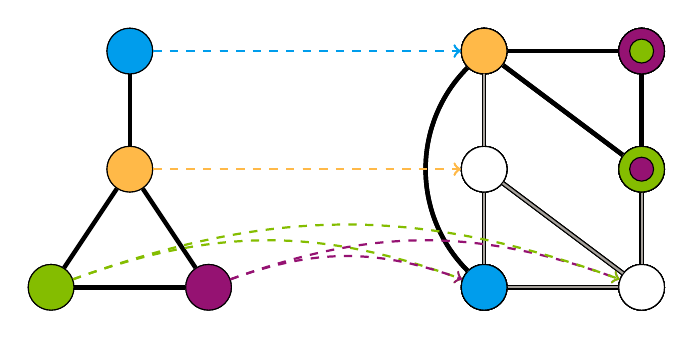
\begin{tikzpicture}
        \node <1> [draw, circle, fill=white, inner sep=4pt, font=\bfseries] (Na) at (1,  0) {\vphantom{1}};
        \node <1> [draw, circle, fill=white, inner sep=4pt, font=\bfseries] (Nb) at (1, -1.5) {\vphantom{1}};
        \node <1> [draw, circle, fill=white, inner sep=4pt, font=\bfseries] (Nc) at (0, -3) {\vphantom{1}};
        \node <1> [draw, circle, fill=white, inner sep=4pt, font=\bfseries] (Nd) at (2, -3) {\vphantom{1}};

        \node <2-8> [draw, circle, fill=uofgcobalt, inner sep=4pt, font=\bfseries] (Na) at (1,  0) {\vphantom{1}};
        \node <2-8> [draw, circle, fill=uofgpumpkin, inner sep=4pt, font=\bfseries] (Nb) at (1, -1.5) {\vphantom{1}};
        \node <2-8> [draw, circle, fill=uofglawn, inner sep=4pt, font=\bfseries] (Nc) at (0, -3) {\vphantom{1}};
        \node <2-8> [draw, circle, fill=uofgthistle, inner sep=4pt, font=\bfseries] (Nd) at (2, -3) {\vphantom{1}};

        \draw [ultra thick] (Na) -- (Nb);
        \draw [ultra thick] (Nb) -- (Nc);
        \draw [ultra thick] (Nc) -- (Nd);
        \draw [ultra thick] (Nb) -- (Nd);

        \node <1> [draw, circle, fill=white, inner sep=4pt, font=\bfseries] (N1) at (5.5,  0) {\vphantom{1}};
        \node <1> [draw, circle, fill=white, inner sep=4pt, font=\bfseries] (N2) at (7.5,  0) {\vphantom{1}};
        \node <1> [draw, circle, fill=white, inner sep=4pt, font=\bfseries] (N3) at (5.5, -1.5) {\vphantom{1}};
        \node <1> [draw, circle, fill=white, inner sep=4pt, font=\bfseries] (N4) at (7.5, -1.5) {\vphantom{1}};
        \node <1> [draw, circle, fill=white, inner sep=4pt, font=\bfseries] (N5) at (5.5, -3) {\vphantom{1}};
        \node <1> [draw, circle, fill=white, inner sep=4pt, font=\bfseries] (N6) at (7.5, -3) {\vphantom{1}};

        \node <2> [draw, circle, fill=uofgcobalt, inner sep=4pt, font=\bfseries] (N1) at (5.5,  0) {\vphantom{1}};
        \node <2> [draw, circle, fill=white, inner sep=4pt, font=\bfseries] (N2) at (7.5,  0) {\vphantom{1}};
        \node <2> [draw, circle, fill=uofgpumpkin, inner sep=4pt, font=\bfseries] (N3) at (5.5, -1.5) {\vphantom{1}};
        \node <2> [draw, circle, fill=white, inner sep=4pt, font=\bfseries] (N4) at (7.5, -1.5) {\vphantom{1}};
        \node <2> [draw, circle, fill=uofglawn, inner sep=4pt, font=\bfseries] (N5) at (5.5, -3) {\vphantom{1}};
        \node <2> [draw, circle, fill=uofgthistle, inner sep=4pt, font=\bfseries] (N6) at (7.5, -3) {\vphantom{1}};

        \node <3> [draw, circle, fill=uofgcobalt, inner sep=4pt, font=\bfseries] (N1) at (5.5,  0) {\vphantom{1}};
        \node <3> [draw, circle, fill=white, inner sep=4pt, font=\bfseries] (N2) at (7.5,  0) {\vphantom{1}};
        \node <3> [draw, circle, fill=uofgpumpkin, inner sep=4pt, font=\bfseries] (N3) at (5.5, -1.5) {\vphantom{1}};
        \node <3> [draw, circle, fill=white, inner sep=4pt, font=\bfseries] (N4) at (7.5, -1.5) {\vphantom{1}};
        \node <3> [draw, circle, fill=uofgthistle, inner sep=4pt, font=\bfseries] (N5) at (5.5, -3) {\vphantom{1}};
        \node <3> [draw, circle, fill=uofglawn, inner sep=4pt, font=\bfseries] (N6) at (7.5, -3) {\vphantom{1}};

        \node <4> [draw, circle, fill=uofglawn, inner sep=4pt, font=\bfseries] (N1) at (5.5,  0) {\vphantom{1}};
        \node <4> [draw, circle, fill=uofgthistle, inner sep=1pt, font=\bfseries] (N1b) at (5.5,  0) {\vphantom{1}};
        \node <4> [draw, circle, fill=uofgthistle, inner sep=4pt, font=\bfseries] (N2) at (7.5,  0) {\vphantom{1}};
        \node <4> [draw, circle, fill=uofglawn, inner sep=1pt, font=\bfseries] (N2b) at (7.5,  0) {\vphantom{1}};
        \node <4> [draw, circle, fill=white, inner sep=4pt, font=\bfseries] (N3) at (5.5, -1.5) {\vphantom{1}};
        \node <4> [draw, circle, fill=uofgpumpkin, inner sep=4pt, font=\bfseries] (N4) at (7.5, -1.5) {\vphantom{1}};
        \node <4> [draw, circle, fill=white, inner sep=4pt, font=\bfseries] (N5) at (5.5, -3) {\vphantom{1}};
        \node <4> [draw, circle, fill=uofgcobalt, inner sep=4pt, font=\bfseries] (N6) at (7.5, -3) {\vphantom{1}};

        \node <5> [draw, circle, fill=uofgpumpkin, inner sep=4pt, font=\bfseries] (N1) at (5.5,  0) {\vphantom{1}};
        \node <5> [draw, circle, fill=uofgthistle, inner sep=4pt, font=\bfseries] (N2) at (7.5,  0) {\vphantom{1}};
        \node <5> [draw, circle, fill=uofglawn, inner sep=1pt, font=\bfseries] (N2b) at (7.5,  0) {\vphantom{1}};
        \node <5> [draw, circle, fill=uofgcobalt, inner sep=4pt, font=\bfseries] (N3) at (5.5, -1.5) {\vphantom{1}};
        \node <5> [draw, circle, fill=uofglawn, inner sep=4pt, font=\bfseries] (N4) at (7.5, -1.5) {\vphantom{1}};
        \node <5> [draw, circle, fill=uofgthistle, inner sep=1pt, font=\bfseries] (N4b) at (7.5, -1.5) {\vphantom{1}};
        \node <5> [draw, circle, fill=white, inner sep=4pt, font=\bfseries] (N5) at (5.5, -3) {\vphantom{1}};
        \node <5> [draw, circle, fill=white, inner sep=4pt, font=\bfseries] (N6) at (7.5, -3) {\vphantom{1}};

        \node <6> [draw, circle, fill=white, inner sep=4pt, font=\bfseries] (N1) at (5.5,  0) {\vphantom{1}};
        \node <6> [draw, circle, fill=white, inner sep=4pt, font=\bfseries] (N2) at (7.5,  0) {\vphantom{1}};
        \node <6> [draw, circle, fill=uofgthistle, inner sep=4pt, font=\bfseries] (N3) at (5.5, -1.5) {\vphantom{1}};
        \node <6> [draw, circle, fill=uofglawn, inner sep=1pt, font=\bfseries] (N3b) at (5.5, -1.5) {\vphantom{1}};
        \node <6> [draw, circle, fill=uofgcobalt, inner sep=4pt, font=\bfseries] (N4) at (7.5, -1.5) {\vphantom{1}};
        \node <6> [draw, circle, fill=uofglawn, inner sep=4pt, font=\bfseries] (N5) at (5.5, -3) {\vphantom{1}};
        \node <6> [draw, circle, fill=uofgthistle, inner sep=1pt, font=\bfseries] (N5b) at (5.5, -3) {\vphantom{1}};
        \node <6> [draw, circle, fill=uofgpumpkin, inner sep=4pt, font=\bfseries] (N6) at (7.5, -3) {\vphantom{1}};

        \node <7> [draw, circle, fill=uofgcobalt, inner sep=4pt, font=\bfseries] (N1) at (5.5,  0) {\vphantom{1}};
        \node <7> [draw, circle, fill=white, inner sep=4pt, font=\bfseries] (N2) at (7.5,  0) {\vphantom{1}};
        \node <7> [draw, circle, fill=uofglawn, inner sep=4pt, font=\bfseries] (N3) at (5.5, -1.5) {\vphantom{1}};
        \node <7> [draw, circle, fill=uofgthistle, inner sep=1pt, font=\bfseries] (N3b) at (5.5, -1.5) {\vphantom{1}};
        \node <7> [draw, circle, fill=white, inner sep=4pt, font=\bfseries] (N4) at (7.5, -1.5) {\vphantom{1}};
        \node <7> [draw, circle, fill=uofgpumpkin, inner sep=4pt, font=\bfseries] (N5) at (5.5, -3) {\vphantom{1}};
        \node <7> [draw, circle, fill=uofgthistle, inner sep=4pt, font=\bfseries] (N6) at (7.5, -3) {\vphantom{1}};
        \node <7> [draw, circle, fill=uofglawn, inner sep=1pt, font=\bfseries] (N6b) at (7.5, -3) {\vphantom{1}};

        \node <8> [draw, circle, fill=uofgpumpkin, inner sep=4pt, font=\bfseries] (N1) at (5.5,  0) {\vphantom{1}};
        \node <8> [draw, circle, fill=uofgthistle, inner sep=4pt, font=\bfseries] (N2) at (7.5,  0) {\vphantom{1}};
        \node <8> [draw, circle, fill=uofglawn, inner sep=1pt, font=\bfseries] (N2b) at (7.5,  0) {\vphantom{1}};
        \node <8> [draw, circle, fill=white, inner sep=4pt, font=\bfseries] (N3) at (5.5, -1.5) {\vphantom{1}};
        \node <8> [draw, circle, fill=uofglawn, inner sep=4pt, font=\bfseries] (N4) at (7.5, -1.5) {\vphantom{1}};
        \node <8> [draw, circle, fill=uofgthistle, inner sep=1pt, font=\bfseries] (N4b) at (7.5, -1.5) {\vphantom{1}};
        \node <8> [draw, circle, fill=uofgcobalt, inner sep=4pt, font=\bfseries] (N5) at (5.5, -3) {\vphantom{1}};
        \node <8> [draw, circle, fill=white, inner sep=4pt, font=\bfseries] (N6) at (7.5, -3) {\vphantom{1}};

        \draw <1> [thick, color=uofgsandstone!50] (N1) -- (N2);
        \draw <1> [thick, color=uofgsandstone!50] (N1) -- (N3);
        \draw <1> [thick, color=uofgsandstone!50] (N1) -- (N4);
        \draw <1> [thick, color=uofgsandstone!50] (N2) -- (N4);
        \draw <1> [thick, color=uofgsandstone!50] (N3) -- (N5);
        \draw <1> [thick, color=uofgsandstone!50] (N3) -- (N6);
        \draw <1> [thick, color=uofgsandstone!50] (N4) -- (N6);
        \draw <1> [thick, color=uofgsandstone!50] (N5) -- (N6);
        \draw <1> [thick, color=uofgsandstone!50] (N1) to [in=135, out=225] (N5);

        \draw <2-3> [thick, color=uofgsandstone!50] (N1) -- (N2);
        \draw <2-3> [ultra thick] (N1) -- (N3);
        \draw <2-3> [thick, color=uofgsandstone!50] (N1) -- (N4);
        \draw <2-3> [thick, color=uofgsandstone!50] (N2) -- (N4);
        \draw <2-3> [ultra thick] (N3) -- (N5);
        \draw <2-3> [ultra thick] (N3) -- (N6);
        \draw <2-3> [thick, color=uofgsandstone!50] (N4) -- (N6);
        \draw <2-3> [ultra thick] (N5) -- (N6);
        \draw <2-3> [thick, color=uofgsandstone!50] (N1) to [in=135, out=225] (N5);

        \draw <4> [ultra thick] (N1) -- (N2);
        \draw <4> [thick, color=uofgsandstone!50] (N1) -- (N3);
        \draw <4> [ultra thick] (N1) -- (N4);
        \draw <4> [ultra thick] (N2) -- (N4);
        \draw <4> [thick, color=uofgsandstone!50] (N3) -- (N5);
        \draw <4> [thick, color=uofgsandstone!50] (N3) -- (N6);
        \draw <4> [ultra thick] (N4) -- (N6);
        \draw <4> [thick, color=uofgsandstone!50] (N5) -- (N6);
        \draw <4> [thick, color=uofgsandstone!50] (N1) to [in=135, out=225] (N5);

        \draw <5> [ultra thick] (N1) -- (N2);
        \draw <5> [ultra thick] (N1) -- (N3);
        \draw <5> [ultra thick] (N1) -- (N4);
        \draw <5> [ultra thick] (N2) -- (N4);
        \draw <5> [thick, color=uofgsandstone!50] (N3) -- (N5);
        \draw <5> [thick, color=uofgsandstone!50] (N3) -- (N6);
        \draw <5> [thick, color=uofgsandstone!50] (N4) -- (N6);
        \draw <5> [thick, color=uofgsandstone!50] (N5) -- (N6);
        \draw <5> [thick, color=uofgsandstone!50] (N1) to [in=135, out=225] (N5);

        \draw <6> [thick, color=uofgsandstone!50] (N1) -- (N2);
        \draw <6> [thick, color=uofgsandstone!50] (N1) -- (N3);
        \draw <6> [thick, color=uofgsandstone!50] (N1) -- (N4);
        \draw <6> [thick, color=uofgsandstone!50] (N2) -- (N4);
        \draw <6> [ultra thick] (N3) -- (N5);
        \draw <6> [ultra thick] (N3) -- (N6);
        \draw <6> [ultra thick] (N4) -- (N6);
        \draw <6> [ultra thick] (N5) -- (N6);
        \draw <6> [thick, color=uofgsandstone!50] (N1) to [in=135, out=225] (N5);

        \draw <7> [thick, color=uofgsandstone!50] (N1) -- (N2);
        \draw <7> [thick, color=uofgsandstone!50] (N1) -- (N3);
        \draw <7> [thick, color=uofgsandstone!50] (N1) -- (N4);
        \draw <7> [thick, color=uofgsandstone!50] (N2) -- (N4);
        \draw <7> [ultra thick] (N3) -- (N5);
        \draw <7> [ultra thick] (N3) -- (N6);
        \draw <7> [thick, color=uofgsandstone!50] (N4) -- (N6);
        \draw <7> [ultra thick] (N5) -- (N6);
        \draw <7> [ultra thick] (N1) to [in=135, out=225] (N5);

        \draw <8> [ultra thick] (N1) -- (N2);
        \draw <8> [thick, color=uofgsandstone!50] (N1) -- (N3);
        \draw <8> [ultra thick] (N1) -- (N4);
        \draw <8> [ultra thick] (N2) -- (N4);
        \draw <8> [thick, color=uofgsandstone!50] (N3) -- (N5);
        \draw <8> [thick, color=uofgsandstone!50] (N3) -- (N6);
        \draw <8> [thick, color=uofgsandstone!50] (N4) -- (N6);
        \draw <8> [thick, color=uofgsandstone!50] (N5) -- (N6);
        \draw <8> [ultra thick] (N1) to [in=135, out=225] (N5);

        \draw <2> [thick, dashed, color=uofgcobalt, arrows=->] (Na) to (N1);
        \draw <2> [thick, dashed, color=uofgpumpkin, arrows=->] (Nb) to (N3);
        \draw <2> [thick, dashed, color=uofglawn, arrows=->] (Nc) to [out=20, in=160] (N5);
        \draw <2> [thick, dashed, color=uofgthistle, arrows=->] (Nd) to [out=20, in=160] (N6);

        \draw <3> [thick, dashed, color=uofgcobalt, arrows=->] (Na) to (N1);
        \draw <3> [thick, dashed, color=uofgpumpkin, arrows=->] (Nb) to (N3);
        \draw <3> [thick, dashed, color=uofglawn, arrows=->] (Nc) to [out=20, in=160] (N6);
        \draw <3> [thick, dashed, color=uofgthistle, arrows=->] (Nd) to [out=20, in=160] (N5);
    \end{tikzpicture}}

  \begin{itemize}
  \item
    Find the
%%% Trying to do consistent highlighting in our slides with \alert commands... -JN
%       \emph{pattern}
    \alertblue{pattern}
    inside the
%       \emph{target}
    \alertblue{target}

  \item
    Applications in compilers, biochemistry, model checking, pattern recognition, \ldots

  \item
    Often want to find
%       \emph{all}
    \alertred{all}
    matches
\end{itemize}
\end{frame}

\begin{frame}[t]{Subgraph Isomorphism in Pseudo-Boolean Form}
Each pattern vertex gets a target vertex: \begin{align*}
    \sum_{t \in \vertexset(T)} x_{p{,}t}  & = 1 && p \in \vertexset(P)
\end{align*}\pause
Each target vertex may be used at most once:\begin{align*}
    \sum_{p \in \vertexset(P)} -x_{p{,}t} & \ge -1 && t \in \vertexset(T)
\end{align*}\pause
Adjacency constraints, if $p$ is mapped to $t$, then $p$'s neighbours must
be mapped to $t$'s neighbours: \begin{align*}
    \overline{x}_{p{,}t} + \sum_{u \in \neighbourhood(t)} x_{q{,}u} & \ge 1 && p \in \vertexset(P),~q \in \neighbourhood(p),~t \in \vertexset(T)
\end{align*}
\end{frame}

\begin{frame}[fragile]{Degree Reasoning in Cutting Planes}
%     A pattern
  Pattern
  vertex $p$ of degree $\degree(p)$ can never be mapped to
%    a
  target vertex $t$ of degree
%     $\degree(p)-1$ or lower
  $< \degree(p)$
  in any subgraph isomorphism.

  \medskip

  Observe
  $\neighbourhood(\textcolor{uofgcobalt}{p})
  = \{ \textcolor{uofglawn}{q}, \textcolor{uofglawn}{r}, \textcolor{uofglawn}{s} \}$
  and
  $\neighbourhood(\textcolor{uofgcobalt}{t})
  = \{ \textcolor{uofgthistle}{u}, \textcolor{uofgthistle}{v} \}$.

  \medskip

  We wish to derive $\overline{x}_{\textcolor{uofgcobalt}{p}{,}\textcolor{uofgcobalt}{t}} \ge 1$.
\begin{tikzpicture}[overlay,remember picture]
    \node [anchor=center, text depth=0.5cm, xshift=4.8cm, yshift=2.3cm]
    at (current page.center) {
        \begin{minipage}[t]{0.3\paperwidth}\raggedright
            \begin{tikzpicture}
                \node [draw, circle, fill=white, inner sep=2.5pt, font=\scriptsize] (NO) at (0, 0.7) {\phantom{1}};
                \node [anchor=center, font=\scriptsize] at (NO) {o};
                \node [draw, circle, fill=uofgcobalt, inner sep=2.5pt, font=\scriptsize] (NP) at (0, 0) {\phantom{1}};
                \node [anchor=center, font=\scriptsize] at (NP) {p};
                \node [draw, circle, fill=uofglawn, inner sep=2.5pt, font=\scriptsize] (NQ) at (0.7, 0.7) {\phantom{1}};
                \node [anchor=center, font=\scriptsize] at (NQ) {q};
                \node [draw, circle, fill=uofglawn, inner sep=2.5pt, font=\scriptsize] (NR) at (0.7, 0) {\phantom{1}};
                \node [anchor=center, font=\scriptsize] at (NR) {r};
                \node [draw, circle, fill=uofglawn, inner sep=2.5pt, font=\scriptsize] (NS) at (0.7, -0.7) {\phantom{1}};
                \node [anchor=center, font=\scriptsize] at (NS) {s};
                \draw (NO) -- (NQ);
                \draw (NP) -- (NQ);
                \draw (NP) -- (NR);
                \draw (NP) -- (NS);
                \draw (NQ) -- (NR);
                \draw (NR) -- (NS);

                \node [draw, circle, fill=uofgcobalt, inner sep=2.5pt, font=\scriptsize] (NT) at (1.75, 0) {\phantom{1}};
                \node [anchor=center, font=\scriptsize] at (NT) {t};
                \node [draw, circle, fill=uofgthistle, inner sep=2.5pt, font=\scriptsize] (NU) at (2.45, 0.7) {\phantom{1}};
                \node [anchor=center, font=\scriptsize] at (NU) {u};
                \node [draw, circle, fill=uofgthistle, inner sep=2.5pt, font=\scriptsize] (NV) at (2.45, 0) {\phantom{1}};
                \node [anchor=center, font=\scriptsize] at (NV) {v};
                \node [draw, circle, fill=white, inner sep=2.5pt, font=\scriptsize] (NX) at (3.15, 0.7) {\phantom{1}};
                \node [anchor=center, font=\scriptsize] at (NX) {x};
                \node [draw, circle, fill=white, inner sep=2.5pt, font=\scriptsize] (NY) at (3.15, 0) {\phantom{1}};
                \node [anchor=center, font=\scriptsize] at (NY) {y};
                \node [draw, circle, fill=white, inner sep=2.5pt, font=\scriptsize] (NZ) at (3.15, -0.7) {\phantom{1}};
                \node [anchor=center, font=\scriptsize] at (NZ) {z};
                \draw (NT) -- (NU);
                \draw (NT) -- (NV);
                \draw (NU) -- (NV);
                \draw (NU) -- (NX);
                \draw (NU) -- (NY);
                \draw (NV) -- (NY);
                \draw (NX) -- (NY);
                \draw (NY) -- (NZ);
                \draw (NV) -- (NZ);
            \end{tikzpicture}
        \end{minipage}
    };
\end{tikzpicture}
\end{frame}

\begin{frame}[fragile]{Degree Reasoning in Cutting Planes}
\begin{align*}
    &\textnormal{Adjacency:}&\overline{x}_{\textcolor{uofgcobalt}{p}{,}\textcolor{uofgcobalt}{t}} + x_{\textcolor{uofglawn}{q}{,}\textcolor{uofgthistle}{u}} + x_{\textcolor{uofglawn}{q}{,}\textcolor{uofgthistle}{v}} &\ge\phantom{-}1
    \hspace{0.3\textwidth} %% Leave space for tikz image
    \\
    &&\overline{x}_{\textcolor{uofgcobalt}{p}{,}\textcolor{uofgcobalt}{t}} + x_{\textcolor{uofglawn}{r}{,}\textcolor{uofgthistle}{u}} + x_{\textcolor{uofglawn}{r}{,}\textcolor{uofgthistle}{v}} &\ge \phantom{-}1 \\
    &&\overline{x}_{\textcolor{uofgcobalt}{p}{,}\textcolor{uofgcobalt}{t}} + x_{\textcolor{uofglawn}{s}{,}\textcolor{uofgthistle}{u}} + x_{\textcolor{uofglawn}{s}{,}\textcolor{uofgthistle}{v}} &\ge \phantom{-}1 \\
     &\textnormal{Injectivity:}   &-x_{o{,}\textcolor{uofgthistle}{u}} + -x_{\textcolor{uofgcobalt}{p}{,}\textcolor{uofgthistle}{u}} + -x_{\textcolor{uofglawn}{q}{,}\textcolor{uofgthistle}{u}} + -x_{\textcolor{uofglawn}{r}{,}\textcolor{uofgthistle}{u}} + -x_{\textcolor{uofglawn}{s}{,}\textcolor{uofgthistle}{u}} &\ge -1 \\
        &&-x_{o{,}\textcolor{uofgthistle}{v}} + -x_{\textcolor{uofgcobalt}{p}{,}\textcolor{uofgthistle}{v}} + -x_{\textcolor{uofglawn}{q}{,}\textcolor{uofgthistle}{v}} + -x_{\textcolor{uofglawn}{r}{,}\textcolor{uofgthistle}{v}} + -x_{\textcolor{uofglawn}{s}{,}\textcolor{uofgthistle}{v}} &\ge -1 \\
    &\textnormal{Literal axioms:}&x_{o{,}\textcolor{uofgthistle}{u}} &\ge \phantom{-}0 \\
    &&x_{o{,}\textcolor{uofgthistle}{v}} &\ge\phantom{-} 0 \\
    &&x_{\textcolor{uofgcobalt}{p}{,}\textcolor{uofgthistle}{u}} &\ge\phantom{-} 0 \\
    &&x_{\textcolor{uofgcobalt}{p}{,}\textcolor{uofgthistle}{v}} &\ge\phantom{-} 0 \\
    &\rlap{\text{Add these together \only<.(1)>{\dots}\only<+(1)->{and divide by 3 to get}}} \\
    &&\only<.>{3\cdot}\overline{x}_{\textcolor{uofgcobalt}{p}{,}\textcolor{uofgcobalt}{t}} &\ge\phantom{-} 1
  \end{align*}
\begin{tikzpicture}[overlay,remember picture]
    \node [anchor=center, text depth=0.5cm, xshift=4.8cm, yshift=2.3cm]
    at (current page.center) {
        \begin{minipage}[t]{0.3\paperwidth}\raggedright
            \begin{tikzpicture}
                \node [draw, circle, fill=white, inner sep=2.5pt, font=\scriptsize] (NO) at (0, 0.7) {\phantom{1}};
                \node [anchor=center, font=\scriptsize] at (NO) {o};
                \node [draw, circle, fill=uofgcobalt, inner sep=2.5pt, font=\scriptsize] (NP) at (0, 0) {\phantom{1}};
                \node [anchor=center, font=\scriptsize] at (NP) {p};
                \node [draw, circle, fill=uofglawn, inner sep=2.5pt, font=\scriptsize] (NQ) at (0.7, 0.7) {\phantom{1}};
                \node [anchor=center, font=\scriptsize] at (NQ) {q};
                \node [draw, circle, fill=uofglawn, inner sep=2.5pt, font=\scriptsize] (NR) at (0.7, 0) {\phantom{1}};
                \node [anchor=center, font=\scriptsize] at (NR) {r};
                \node [draw, circle, fill=uofglawn, inner sep=2.5pt, font=\scriptsize] (NS) at (0.7, -0.7) {\phantom{1}};
                \node [anchor=center, font=\scriptsize] at (NS) {s};
                \draw (NO) -- (NQ);
                \draw (NP) -- (NQ);
                \draw (NP) -- (NR);
                \draw (NP) -- (NS);
                \draw (NQ) -- (NR);
                \draw (NR) -- (NS);

                \node [draw, circle, fill=uofgcobalt, inner sep=2.5pt, font=\scriptsize] (NT) at (1.75, 0) {\phantom{1}};
                \node [anchor=center, font=\scriptsize] at (NT) {t};
                \node [draw, circle, fill=uofgthistle, inner sep=2.5pt, font=\scriptsize] (NU) at (2.45, 0.7) {\phantom{1}};
                \node [anchor=center, font=\scriptsize] at (NU) {u};
                \node [draw, circle, fill=uofgthistle, inner sep=2.5pt, font=\scriptsize] (NV) at (2.45, 0) {\phantom{1}};
                \node [anchor=center, font=\scriptsize] at (NV) {v};
                \node [draw, circle, fill=white, inner sep=2.5pt, font=\scriptsize] (NX) at (3.15, 0.7) {\phantom{1}};
                \node [anchor=center, font=\scriptsize] at (NX) {x};
                \node [draw, circle, fill=white, inner sep=2.5pt, font=\scriptsize] (NY) at (3.15, 0) {\phantom{1}};
                \node [anchor=center, font=\scriptsize] at (NY) {y};
                \node [draw, circle, fill=white, inner sep=2.5pt, font=\scriptsize] (NZ) at (3.15, -0.7) {\phantom{1}};
                \node [anchor=center, font=\scriptsize] at (NZ) {z};
                \draw (NT) -- (NU);
                \draw (NT) -- (NV);
                \draw (NU) -- (NV);
                \draw (NU) -- (NX);
                \draw (NU) -- (NY);
                \draw (NV) -- (NY);
                \draw (NX) -- (NY);
                \draw (NY) -- (NZ);
                \draw (NV) -- (NZ);
            \end{tikzpicture}
        \end{minipage}
    };
\end{tikzpicture}
\end{frame}

%%% make sure subscripts all take integer number of x's worth of space
\newcommand\subhere[1]{\makebox[\widthof{xxxx}]{$_{#1}$}}

\begin{frame}[fragile]{Degree Reasoning in \veripb}
\begin{Verbatim}[commandchars=\\\{\},codes={\catcode`$=3\catcode`^=7\catcode`_=8}]
pol \textcolor{uofglawn}{18}\subhere{\textcolor{uofgheather}{p{\sim}t{:}q}} \textcolor{uofglawn}{19}\subhere{\textcolor{uofgheather}{p{\sim}t{:}r}} + \textcolor{uofglawn}{20}\subhere{\textcolor{uofgheather}{p{\sim}t{:}s}} +  \textcolor{uofgcobalt}{* sum adjacency constraints}
  \textcolor{uofglawn}{12}\subhere{\textcolor{uofgheather}{inj(u)}} + \textcolor{uofglawn}{13}\subhere{\textcolor{uofgheather}{inj(v)}} +           \textcolor{uofgcobalt}{* sum injectivity constraints}
  xo\textunderscore{}u + xo\textunderscore{}v +               \textcolor{uofgcobalt}{* cancel stray xo\textunderscore{}*}
  xp\textunderscore{}u + xp\textunderscore{}v +               \textcolor{uofgcobalt}{* cancel stray xp\textunderscore{}*}
  \textcolor{uofgpumpkin}{3} d                         \textcolor{uofgcobalt}{* divide, and we're done}
\end{Verbatim}

\medskip

Or we can ask \veripb to do the last bit of simplification automatically:

\medskip

\begin{Verbatim}[commandchars=\\\{\},codes={\catcode`$=3\catcode`^=7\catcode`_=8}]
pol \textcolor{uofglawn}{18}\subhere{\textcolor{uofgheather}{p{\sim}t{:}q}} \textcolor{uofglawn}{19}\subhere{\textcolor{uofgheather}{p{\sim}t{:}r}} + \textcolor{uofglawn}{20}\subhere{\textcolor{uofgheather}{p{\sim}t{:}s}} +  \textcolor{uofgcobalt}{* sum adjacency constraints}
  \textcolor{uofglawn}{12}\subhere{\textcolor{uofgheather}{inj(u)}} + \textcolor{uofglawn}{13}\subhere{\textcolor{uofgheather}{inj(v)}} +           \textcolor{uofgcobalt}{* sum injectivity constraints}
ia \textcolor{uofgpillarbox}{-1} : 1 ~xp\textunderscore{}t >= 1 ;        \textcolor{uofgcobalt}{* desired conclusion is implied}
\end{Verbatim}
%%% Just experimenting above, Ciaran --- feel free to change back -JN
%   * and simplify the above%
%
\end{frame}

\begin{frame}{Other Forms of Reasoning}
We can also log all of the other things state of the art subgraph solvers do:
\begin{itemize}
\item
  Injectivity reasoning and filtering,
\item
  Distance filtering,
\item
  Neighbourhood degree sequences,
\item
  Path filtering,
\item
  Supplemental graphs.
\end{itemize}

\medskip

\uncover<2->{
  Proof steps are ``efficient'' using cutting planes:
  \begin{itemize}
  \item
%       The length of the proof steps are no worse than the time
%       complexity of the reasoning algorithms
    Length of proof $\approx$
    time complexity of the reasoning algorithms.

  \item
    Most proof steps require only trivial additional computations.
  \end{itemize}}
\end{frame}

\begin{frame}{Code}
  \begin{center}
    \url{https://github.com/ciaranm/glasgow-subgraph-solver}
  \end{center}
  \medskip
  Released under MIT Licence.
\end{frame}

\section{End-to-End Verification}

\subsection{Gocht, McCreesh, Myreen, Nordstr\"om, Oertel, Tan: End-to-End Verification for Subgraph Solving, AAAI 2024}

\begin{frame}{Reducing the Trust Base}
    \begin{center}
        \begin{tikzpicture}
            \node (solver) [ inner xsep=4em, inner ysep=2.5em, draw, rounded corners=3pt] { Solver };
            \node (elaborator) [ right=2cm of solver.north east, anchor=north west, inner
            xsep=0.25em, draw, rounded corners=3pt, minimum height=12em, text width=5em, text centered] {
                \only<1>{Checker}\only<2->{Elaborator} };
            \node (verifiedchecker) [ right=2cm of elaborator.north east, anchor=north west, inner
                xsep=0.25em, draw, rounded corners=3pt, minimum height=8em, text width=4em, text
                centered, yshift=-2cm, visible on=<3->] { Verified Checker };

            \node (print) [anchor=south, above=0cm of solver.south] { added print statements };
            \draw [dotted] (solver.west|-print.north) -- (solver.east|-print.north);

            \draw [->, thick] (solver.east) -- (solver.east -| elaborator.west) coordinate [midway]
            (solutionmid) node [above, midway] { Answer };

            \draw [->, thick, rounded corners=3pt] (solver.south) -- (solver.south |- elaborator.west) -- (elaborator.west) coordinate [midway] (proofmid);

            \coordinate (prooflabel) at (proofmid-|solutionmid); \node [above=0cm of prooflabel] { Proof };

            \coordinate [right=2cm of verifiedchecker.east] (verified);
            \draw [->, thick, visible on=<3>] (verifiedchecker.east) -- (verified)
                node [above, midway] { \textcolor{uofglawn}{\ding{51}} or \textcolor{uofgpillarbox}{\ding{55}} }
                node [below, midway, text centered, text width=5em] { Trusted Answer };
            \draw [->, thick, visible on=<4>] (verifiedchecker.east) -- (verified)
                node [above, midway] { \textcolor{uofglawn}{\ding{51}} or \textcolor{uofgpillarbox}{\ding{55}} }
                node [below, midway, text centered, text width=5em] { Trusted Answer in Graph Language };

            \coordinate [left=1.5cm of solver.west] (input);
            \draw [->, thick] (input) -- (solver.west) coordinate [midway] (inputmid) node [above, midway] { Input };

            \coordinate (verifiedcheckertopleft) at ($(verifiedchecker.west)+($(0cm,1.2cm)$)$);
            \draw [->, thick, visible on=<2->] (elaborator.east |- verifiedcheckertopleft) --
            (verifiedcheckertopleft) node [above, midway, text width=4em, text centered] { Answer };
            \draw [->, thick, visible on=<2->] (elaborator.east |- verifiedchecker.west) -- (verifiedchecker.west) node [above, midway, text width=4em, text centered] { Kernel Proof };

            \coordinate (elaboratorbotleft) at ($(elaborator.west)+($(elaborator.west)-(solver.east-|elaborator.west)$)$);
            \coordinate (verifiedcheckerbotleft) at ($(verifiedchecker.west)+($(0cm,-1.2cm)$)$);

            \coordinate (elaboratortopright) at ($(elaborator.east)+($(verifiedcheckertopleft)-(verifiedchecker.west)$)$);
            \draw [->, thick] (elaboratortopright) -- (elaboratortopright-|verifiedchecker.west)
                node [above, midway] { \textcolor{uofglawn}{\ding{51}} or \textcolor{uofgpillarbox}{\ding{55}} };

            \coordinate (solverstart) at ($(solver.south)!0.75!(solver.south west)$);
            \coordinate (checkerbotleft) at ($(elaborator.west)+($(elaborator.west)-(solver.east-|elaborator.west)$)$);
            \draw [->, thick, rounded corners=3pt] (solverstart) -- (solverstart |- checkerbotleft) -- (checkerbotleft)
            coordinate [midway] (altinputmid);

            \coordinate (encinputlabel) at (altinputmid-|solutionmid);
            \node [above=0cm of encinputlabel, xshift=-0.5cm] { Encoded Input };

            \draw [->, thick, rounded corners=3pt, visible on=<3>] (solverstart) -- (solverstart |- verifiedcheckerbotleft) -- (verifiedcheckerbotleft);
            \draw [->, thick, rounded corners=3pt, visible on=<4>] ($(inputmid)+(-0.2,0)$) --
            (inputmid) -- (inputmid |- verifiedcheckerbotleft) -- (verifiedcheckerbotleft)
            coordinate [midway] (verinputmid);

            \coordinate (verinputlabel) at (verinputmid-|solutionmid);
            \node [above=0cm of verinputlabel, xshift=-0.5cm, visible on=<4>] { Verified Input };
        \end{tikzpicture}
    \end{center}
\end{frame}

\begin{frame}[fragile]{End-to-End Verification of Subgraph-Finding}\vspace*{-0.3cm}
\begin{Verbatim}
$ glasgow_clique_solver brock200_4.clq --prove brock200_4 --proof-names --recover-proof-enc
omega = 17
clique = 12 19 28 29 38 54 65 71 79 93 117 127 139 161 165 186 192

$ veripb proof.opb proof.pbp
Verification succeeded.

$ grep conclusion proof.pbp
conclusion BOUNDS 183 183

$ cake_pb_clique brock200_4.clq > brock200_4.verifiedopb

$ veripb proof.verifiedopb proof.pbp --proofOutput proof.corepb
Verification succeeded.

$ cake_pb_clique brock200_4.clq proof.corepb
s VERIFIED MAX CLIQUE SIZE |CLIQUE| = 17
\end{Verbatim}
\end{frame}

\begin{frame}{What Exactly are we Verifying?}
    \only<1>{
    \begin{holthmenv}
    \HOLConst{is_clique}\;\HOLFreeVar{vs}\;(\HOLFreeVar{v}\HOLSymConst{,}\HOLFreeVar{e})\;\HOLTokenDefEquality{}\\
    \;\;\HOLFreeVar{vs}\;\HOLSymConst{\HOLTokenSubset{}}\;\HOLcount{\HOLFreeVar{v}}\;\HOLSymConst{\HOLTokenConj{}}\\
    \;\;\HOLSymConst{\HOLTokenForall{}}\HOLBoundVar{x}\;\HOLBoundVar{y}.\;\HOLBoundVar{x}\;\HOLSymConst{\HOLTokenIn{}}\;\HOLFreeVar{vs}\;\HOLSymConst{\HOLTokenConj{}}\;\HOLBoundVar{y}\;\HOLSymConst{\HOLTokenIn{}}\;\HOLFreeVar{vs}\;\HOLSymConst{\HOLTokenConj{}}\;\HOLBoundVar{x}\;\HOLSymConst{\HOLTokenNotEqual{}}\;\HOLBoundVar{y}\;\HOLSymConst{\HOLTokenImp{}}\;\HOLConst{is_edge}\;\HOLFreeVar{e}\;\HOLBoundVar{x}\;\HOLBoundVar{y}
    \end{holthmenv}

    \begin{holthmenv}
    \HOLConst{max_clique_size}\;\HOLFreeVar{g}\;\HOLTokenDefEquality{}\;\HOLConst{max\ensuremath{_{\text{set}}}}\;\HOLTokenLeftbrace{}\HOLConst{card}\;\HOLBoundVar{vs}\;\HOLTokenBar{}\;\HOLConst{is_clique}\;\HOLBoundVar{vs}\;\HOLFreeVar{g}\HOLTokenRightbrace{}
    \end{holthmenv}
}\only<2>{
\begin{holthmenv}
\HOLConst{clique_eq_str}\;\HOLFreeVar{n}\;\HOLTokenDefEquality{}\;\HOLStringLitDG{s VERIFIED MAX CLIQUE SIZE |CLIQUE| = }\;\HOLSymConst{\^{}}\;\HOLConst{toString}\;\HOLFreeVar{n}\;\HOLSymConst{\^{}}\;\HOLStringLitDG{\HOLTokenBackslash{}n}
\end{holthmenv}

\begin{holthmenv}
\HOLConst{clique_bound_str}\;\HOLFreeVar{l}\;\HOLFreeVar{u}\;\HOLTokenDefEquality{}\\
\;\;\HOLStringLitDG{s VERIFIED MAX CLIQUE SIZE BOUND }\;\HOLSymConst{\^{}}\;\HOLConst{toString}\;\HOLFreeVar{l}\;\HOLSymConst{\^{}}\;\HOLStringLitDG{ <= |CLIQUE| <= }\;\HOLSymConst{\^{}}\;\HOLConst{toString}\;\HOLFreeVar{u}\;\HOLSymConst{\^{}}\;\HOLStringLitDG{\HOLTokenBackslash{}n}
\end{holthmenv}

\begin{holthmenv}
\HOLTokenTurnstile{}\;\HOLConst{cake_pb_clique_run}\;\HOLFreeVar{cl}\;\HOLFreeVar{fs}\;\HOLFreeVar{mc}\;\HOLFreeVar{ms}\;\HOLSymConst{\HOLTokenImp{}}\\
\;\;\;\;\;\HOLConst{machine_sem}\;\HOLFreeVar{mc}\;(\HOLConst{basis_ffi}\;\HOLFreeVar{cl}\;\HOLFreeVar{fs})\;\HOLFreeVar{ms}\;\HOLSymConst{\HOLTokenSubset{}}\\
\;\;\;\;\;\;\;\HOLConst{extend_with_resource_limit}\;\HOLTokenLeftbrace{}\HOLConst{Terminate}\;\HOLConst{Success}\;(\HOLConst{cake_pb_clique_io_events}\;\HOLFreeVar{cl}\;\HOLFreeVar{fs})\HOLTokenRightbrace{}\;\HOLSymConst{\HOLTokenConj{}}\\
\;\;\;\;\;\HOLSymConst{\HOLTokenExists{}}\HOLBoundVar{out}\;\HOLBoundVar{err}.\\
\;\;\;\;\;\;\;\HOLConst{extract_fs}\;\HOLFreeVar{fs}\;(\HOLConst{cake_pb_clique_io_events}\;\HOLFreeVar{cl}\;\HOLFreeVar{fs})\;\HOLSymConst{=}\;\HOLConst{Some}\;(\HOLConst{add_stdout}\;(\HOLConst{add_stderr}\;\HOLFreeVar{fs}\;\HOLBoundVar{err})\;\HOLBoundVar{out})\;\HOLSymConst{\HOLTokenConj{}}\\
\;\;\;\;\;\;\;(\HOLBoundVar{out}\;\HOLSymConst{\HOLTokenNotEqual{}}\;\HOLStringLitDG{}\;\HOLSymConst{\HOLTokenImp{}}\\
\;\;\;\;\;\;\;\;\;\;\HOLSymConst{\HOLTokenExists{}}\HOLBoundVar{g}.\;\HOLConst{get_graph_dimacs}\;\HOLFreeVar{fs}\;(\HOLConst{el}\;\HOLNumLit{1}\;\HOLFreeVar{cl})\;\HOLSymConst{=}\;\HOLConst{Some}\;\HOLBoundVar{g}\;\HOLSymConst{\HOLTokenConj{}}\\
\;\;\;\;\;\;\;\;\;\;\;\;\;\;(\HOLConst{length}\;\HOLFreeVar{cl}\;\HOLSymConst{=}\;\HOLNumLit{2}\;\HOLSymConst{\HOLTokenConj{}}\;\HOLBoundVar{out}\;\HOLSymConst{=}\;\HOLConst{concat}\;(\HOLConst{print_pbf}\;(\HOLConst{full_encode}\;\HOLBoundVar{g}))\;\HOLSymConst{\HOLTokenDisj{}}\\
\;\;\;\;\;\;\;\;\;\;\;\;\;\;\;\HOLConst{length}\;\HOLFreeVar{cl}\;\HOLSymConst{=}\;\HOLNumLit{3}\;\HOLSymConst{\HOLTokenConj{}}\\
\;\;\;\;\;\;\;\;\;\;\;\;\;\;\;\;\;\;\;(\HOLBoundVar{out}\;\HOLSymConst{=}\;\HOLConst{clique_eq_str}\;(\HOLConst{max_clique_size}\;\HOLBoundVar{g})\;\HOLSymConst{\HOLTokenDisj{}}\\
\;\;\;\;\;\;\;\;\;\;\;\;\;\;\;\;\;\;\;\HOLSymConst{\HOLTokenExists{}}\HOLBoundVar{l}\;\HOLBoundVar{u}.\HOLBoundVar{out}\;\HOLSymConst{=}\;\HOLConst{clique_bound_str}\;\HOLBoundVar{l}\;\HOLBoundVar{u}\;\HOLSymConst{\HOLTokenConj{}}\;(\HOLSymConst{\HOLTokenForall{}}\HOLBoundVar{vs}.\;\HOLConst{is_clique}\;\HOLBoundVar{vs}\;\HOLBoundVar{g}\;\HOLSymConst{\HOLTokenImp{}}\;\HOLConst{card}\;\HOLBoundVar{vs}\;\HOLSymConst{\HOLTokenLeq{}}\;\HOLBoundVar{u})\;\HOLSymConst{\HOLTokenConj{}}\\
\;\;\;\;\;\;\;\;\;\;\;\;\;\;\;\;\;\;\;\;\;\;\;\;\;\;\HOLSymConst{\HOLTokenExists{}}\HOLBoundVar{vs}.\;\HOLConst{is_clique}\;\HOLBoundVar{vs}\;\HOLBoundVar{g}\;\HOLSymConst{\HOLTokenConj{}}\;\HOLBoundVar{l}\;\HOLSymConst{\HOLTokenLeq{}}\;\HOLConst{card}\;\HOLBoundVar{vs})))
\end{holthmenv}}
\end{frame}

\begin{frame}{What's Left to Trust?}
    Still have to trust:
    \begin{itemize}
        \item The HOL4 theorem prover.
        \item That the formal HOL model of the CakeML environment corresponds to the
            hardware on which it is run.
        \item HOL definition of what it means to be a maximum clique or a subgraph isomorphism.
        \item Input parsing and output formatting.
    \end{itemize}

    \bigskip

    No need to trust, or even know about:
    \begin{itemize}
        \item How the solver works.
        \item What pseudo-Boolean means.
    \end{itemize}
\end{frame}

\begin{frame}{Code}
  \begin{center}
    \url{https://github.com/ciaranm/glasgow-subgraph-solver}

      \bigskip

    \url{https://gitlab.com/MIAOresearch/software/VeriPB}

      \bigskip

      \url{https://gitlab.com/MIAOresearch/software/CakePB}
  \end{center}
\end{frame}

\section{Constraint Programming}

\subsection{Gocht, McCreesh, Nordstr\"om: An Auditable Constraint Programming Solver, CP 2022}

\begin{frame}{What About Constraint Programming?}
    Non-Boolean variables?

    \medskip

    Constraints?
    \begin{itemize}
    \item Encoding constraints in pseudo-Boolean form?
    \item Justifying inferences?
    \end{itemize}

    \medskip

    Reformulations?
\end{frame}

\begin{frame}[t]{Compiling CP Variables (1/2)}
  Given $A \in \{ -3 \ldots 9 \}$, the direct encoding is:
  \begin{align*}
    a_{{=}-3} + a_{{=}-2} + a_{{=}-1} + a_{{=}0} + a_{{=}1} + a_{{=}2}
    + a_{{=}3} \\ +~a_{{=}4} + a_{{=}5} + a_{{=}6} + a_{{=}7}
    + a_{{=}8} + a_{{=}9} &= 1
  \end{align*}

  \uncover<2->{This doesn't work for large domains\ldots}

  \medskip

  \uncover<3->{
    We could use a binary encoding:
    \begin{align*}
      -16 a_{{\operatorname{neg}}} + 1 a_{{\operatorname{b}}0} + 2 a_{{\operatorname{b}}1} + 4
      a_{{\operatorname{b}}2} + 8 a_{{\operatorname{b}}3}
      &\ge -3
        \qquad
        \textnormal{~and}\\
      16 a_{{\operatorname{neg}}} + -1 a_{{\operatorname{b}}0} + -2 a_{{\operatorname{b}}1} +
      -4 a_{{\operatorname{b}}2} + -8 a_{{\operatorname{b}}3}
      &\ge -9
    \end{align*}
    This doesn't propagate much, but that isn't a problem for proof logging.
  }

  \medskip

  \uncover<4->{
    \alertred{Convention} in what follows:
    \begin{itemize}
    \item
      Upper-case
      \alertblue{$A, B, C$}
      are
      \alertgreen{CP variables};
    \item
      Lower-case
      \alertblue{$a, b, c$}
      are
      \alertgreen{corresponding Boolean variables}
      in PB encoding.
    \end{itemize}
  }

\end{frame}

\begin{frame}[t]{Compiling CP Variables (2/2)}
  We can mix binary and an order encoding!
  Where needed, define:
  \begin{alignat*}{2}
    a_{{\ge}4}
    & \reifequiv -16 a_{{\operatorname{neg}}} + 1 a_{{\operatorname{b}}0} + 2 a_{{\operatorname{b}}1} + 4
    a_{{\operatorname{b}}2} + 8 a_{{\operatorname{b}}3}
    &&\ge 4
    \\
    a_{{\ge}5}
    & \reifequiv -16 a_{{\operatorname{neg}}} + 1 a_{{\operatorname{b}}0} + 2 a_{{\operatorname{b}}1} + 4
    a_{{\operatorname{b}}2} + 8 a_{{\operatorname{b}}3}
    &&\ge 5
    \\
    a_{{=}4}
    & \reifequiv a_{{\ge}4} \land \overline{a}_{{\ge}5}
  \end{alignat*}

  \pause

  When creating
  %%BB (after IJCAI): typo? Should happen whenever  this variable is
  %%introduced, I presume, even when you don't need equality.
  %$a_{{=}i}$,
  $a_{{\ge}i}$,
  also introduce pseudo-Boolean constraints encoding
  \begin{align*}
    a_{{\ge}i} \reifimplrt a_{{\ge}j} \quad \text{and} \quad a_{{\ge}h} \reifimplrt a_{{\ge}i}
  \end{align*}
  for the closest values $j < i < h$ that already exist.

  \medskip
  \pause


  We can do this:
  \begin{itemize}
  \item
    Inside the pseudo-Boolean model, where needed;
  \item
    Otherwise lazily during proof logging.
  \end{itemize}
\end{frame}

\begin{frame}{Compiling Constraints}
  \begin{itemize}
  \item
    Also need to compile every constraint to pseudo-Boolean form.

    \smallskip

  \item
    Doesn't need to be a propagating encoding.

    \smallskip

  \item
    Can use additional variables.
  \end{itemize}
\end{frame}

\begin{frame}{Compiling Linear Inequalities}

%       Given $2A + 3B + 4C \ge 42$, where $A, B, C \in \{ -3 \ldots 9 \}$,

  Given inequality
  \begin{equation*}
    2A + 3B + 4C \ge 42
  \end{equation*}
  where
  $A, B, C \in \{ -3 \ldots 9 \}$,

  \pause
  \medskip

  Encode in pseudo-Boolean form as
  \begin{align*}
    -32 a_{{\operatorname{neg}}} + 2 a_{{\operatorname{b}}0} + 4 a_{{\operatorname{b}}1} + 8
    a_{{\operatorname{b}}2} + 16 a_{{\operatorname{b}}3} \\
    + -48 b_{{\operatorname{neg}}} + 3 b_{{\operatorname{b}}0} + 6
    b_{{\operatorname{b}}1} + 12 b_{{\operatorname{b}}2} + 24 b_{{\operatorname{b}}3}\\
    + -64 c_{{\operatorname{neg}}} + 4 c_{{\operatorname{b}}0} + 8
    c_{{\operatorname{b}}1} + 16 c_{{\operatorname{b}}2} + 32 c_{{\operatorname{b}}3} & \ge 42
  \end{align*}

\end{frame}

\begin{frame}{Compiling Table Constraints}
  Constraints can be specified
%     \emph{extensionally}
  \alertblue{extensionally}
  as list of feasible tuples,
  called a
%     \emph{table}
  \alertgreen{table}.


  %%% I just don't parse this description... -JN
%     We have to pick one of the tuples from the table, and give it to the associated variables.

  Variable assignments must match some row in table.

  \medskip
  \pause

  Given  table constraint
%       $(A, B, C) \in [(1, 2, 3), (1, 3, 4), (2, 2, 5)]$,
  \begin{equation*}
    (A, B, C) \in [(1, 2, 3), (1, 3, 4), (2, 2, 5)]
  \end{equation*}
  define
  \begin{align*}
    3\overline{t}_{1} + a_{{=}1} + b_{{=}2} + c_{{=}3} \ge 3
    &  %       &\quad \text{i.e.}
    &
      \text{i.e.\ }
      t_{1} \reifimplrt (a_{{=}1} \wedge b_{{=}2} \wedge c_{{=}3})
    \\
    3\overline{t}_{2} + a_{{=}1} + b_{{=}4} + c_{{=}4} \ge 3
    &  %       &\quad \text{i.e.}
    &
      \text{i.e.\ }
      t_{2} \reifimplrt (a_{{=}1} \wedge b_{{=}4} \wedge c_{{=}4})
    \\
    3\overline{t}_{3} + a_{{=}2} + b_{{=}2} + c_{{=}5} \ge 3
    &  %       &\quad \text{i.e.}
    &
      \text{i.e.\ }
      t_{3} \reifimplrt (a_{{=}2} \wedge b_{{=}2} \wedge c_{{=}5})
  \end{align*}
  using
%     a tuple selector variable
  tuple selector variables
  \begin{align*}
    &t_{1} + t_{2} + t_{3} = 1
  \end{align*}

\end{frame}

\begin{frame}{Encoding Constraint Definitions}
%     We already
  Already
  know how to do it for any constraint
%     that has
  with
  a sane encoding using some combination
  of
  \begin{itemize}
  \item
    CNF,
  \item
    Integer linear inequalities,
  \item
    Table constraints,
  \item
    Auxiliary variable.s
  \end{itemize}
  Simplicity is important, propagation strength isn't.
\end{frame}

\begin{frame}{Justifying Search}
    Mostly this works as in earlier examples.

    \medskip

    Restarts are easy.

    \medskip

    No need to justify guesses or decisions, only backtracking.
\end{frame}

\begin{frame}{Justifying Inference}
%
%       Key idea: anything the constraint programming solver knows must follow from
%       unit propagation of guessed assignments in the proof.
%
  \begin{block}{Key idea}
    Anything the constraint programming solver knows must follow from
    \alertred{unit propagation} of guessed assignments on
    \alertred{constraints in proof log}.
  \end{block}

  \pause
  \medskip

  If it follows from unit propagation
%     from
  on
  the encoding, nothing needed

  \medskip

  Some propagators and encodings need RUP steps for inferences
  \begin{itemize}
  \item A lot of propagators are effectively
    ``doing a little bit of lookahead''
    but in an efficient way.
  \end{itemize}

  \medskip
  \pause

  A few need explicit cutting planes justifications
  written to the proof log:
  \begin{itemize}
  \item
    \alertblue{Linear inequalities} just need to multiply and add.
  \item
    \alertblue{All-different} needs a bit more.
  \item
    Might need the help of a good PhD student for some propagators.
  \end{itemize}
\end{frame}

\subsection{Elffers, Gocht, McCreesh, Nordstr\"om: Justifying All Differences Using Pseudo-Boolean Reasoning, AAAI 2020}

\begin{frame}[t]{Justifying All-Different Failures}
%%%
%%% Trying to fine-tune spacing of columns
%%%
  \begin{tabular}%
%%% OLD
%   {r@{\hspace*{0mm}}c@{\hspace*{0.6mm}}c@{\hspace*{0.6mm}}c@{\hspace{0.6mm}}c@{\hspace*{0.6mm}}%
    {r@{\hspace*{0mm}}c@{\hspace*{0.5mm}}c@{\hspace*{0.5mm}}c@{\hspace{0.5mm}}c@{\hspace*{0.5mm}}%
    r@{\hspace*{3mm}}%
%%% OLD
%   r@{\hspace*{0.8mm}}r@{\hspace*{0.8mm}}r@{\hspace*{0.8mm}}r@{\hspace*{0.8mm}}r@{\hspace*{0.8mm}}r@{\hspace*{0.8mm}}r@{\hspace*{0.8mm}}r@{\hspace*{0.8mm}}r@{\hspace*{0.8mm}}%
    r@{\hspace*{0.7mm}}r@{\hspace*{0.7mm}}r@{\hspace*{0.7mm}}r@{\hspace*{0.7mm}}r@{\hspace*{0.7mm}}r@{\hspace*{0.7mm}}r@{\hspace*{0.7mm}}r@{\hspace*{0.7mm}}r@{\hspace*{0.7mm}}%
    ll}
    $V \in \{$
    &
      $1$
    &
    &
    &
      $4$ \hspace*{1.2mm} $5$
    &
      $\}$
    & \phantom{$-v_{{=}1}$}
    &
    & \phantom{$-w_{{=}1}$}
    &
    & \phantom{$-x_{{=}1}$}
    &
    & \phantom{$-y_{{=}1}$}
    &
    & \phantom{$-z_{{=}1}$}
    &
    \\

    $\alertblue<2->{W}
%         \only<2->{{\color{uofgcobalt}W}}
    \in \{$
    &
      \alertred<3>{$1$}
    &
      \alertred<3>{$2$}
    &
      \alertred<3>{$3$}
    &
    &
      $\}$
    &
      $
      \only<1-2>{\phantom{w_{{=}1}}}\only<3->{\alertred<3>{w_{{=}1}}}
      $
    &
      $\only<1-2>{\phantom{+}}\only<3->{\alertred<3>{+}}$
    &
      $\only<1-2>{\phantom{w_{{=}2}}}\only<3->{\alertred<3>{w_{{=}2}}}$
    &
      $\only<1-2>{\phantom{+}}\only<3->{\alertred<3>{+}}$
    &
      $\only<1-2>{\phantom{w_{{=}3}}}\only<3->{\alertred<3>{w_{{=}3}}}$
    &
    &
    &
    &
    &
      $\only<1-2>{\phantom{ \ge \phantom{-}1}}\only<3->{\alertred<3>{ \ge\phantom{-} 1}}$
    &
      \uncover<3->{$[$
      $W\!$ takes some value
      $\!]$}
    \\
    $\alertblue<2->{X} \in \{$
    &
%           $\only<1>{X}\only<2->{{\color{uofgcobalt}X}} \in \{$ &
    &
      $2$
    &
      $3$
    &
    &
      $\}$ &
    &
    &
      $\only<1-3>{\phantom{x_{{=}2}}}\only<4->{x_{{=}2}}$
    &
      $\only<1-3>{\phantom{+}}\only<4->{+}$
    &
      $\only<1-3>{\phantom{x_{{=}3}}}\only<4->{x_{{=}3}}$
    &
    &
    &
    &
    &
      $\only<1-3>{\phantom{ \ge\phantom{-} 1}}\only<4->{ \ge\phantom{-} 1}$
    &
      \uncover<4->{$[$
      $X$ takes some value
      $\!\!\:]$}
    \\
    % $\only<1>{Y}\only<2->{{\color{uofgcobalt}Y}} \in \{$
    $\alertblue<2->{Y} \in \{$
    &
      $1$
    &
    &
      $3$
    &
    &
      $\}$
    &
      $\only<1-3>{\phantom{y_{{=}1}}}\only<4->{y_{{=}1}}$
    &
    &
    &
      $\only<1-3>{\phantom{+}}\only<4->{+}$
    &
      $\only<1-3>{\phantom{y_{{=}3}}}\only<4->{y_{{=}3}}$
    &
    &
    &
    &
    &
      $\only<1-3>{\phantom{ \ge\phantom{-} 1}}\only<4->{ \ge\phantom{-} 1}$
    &
      \uncover<4->{$[$
      $Y$ takes some value
      $]$}
    \\
    % $\only<1>{Z}\only<2->{{\color{uofgcobalt}Z}} \in \{$
    $\alertblue<2->{Z} \in \{$
    &
      $1$
    &
    &
      $3$
    &
    &
      $\}$
    &
      $\only<1-3>{\phantom{z_{{=}1}}}\only<4->{z_{{=}1}}$
    &
    &
    &
      $\only<1-3>{\phantom{+}}\only<4->{+}$
    &
      $\only<1-3>{\phantom{z_{{=}3}}}\only<4->{z_{{=}3}}$
    &
    &
    &
    &
    &
      $\only<1-3>{\phantom{ \ge\phantom{-} 1}}\only<4->{ \ge\phantom{-} 1}$
    &
      \uncover<4->{$[$
      $Z$ takes some value
      $]$}
    \\[0.5cm]

    \only<5->{
    &
      $\rightarrow$
    &
    &
    &
    &
    &
      $-v_{{=}1}$
    &
      $+$
    &
      $-w_{{=}1}$
    &
      $+$
    &
    &
    &
      $-y_{{=}1}$
    &
      $+$
    &
      $-z_{{=}1}$
    &
      $ \ge -1$
    &
      \uncover<5->{$[$
      At most  one variable
      $=1$
      $]$}
    \\

    &
    &
      $\rightarrow$
    &
    &
    &
    &
    &
    &
      $-w_{{=}2}$
    &
      $+$
    &
      $-x_{{=}2}$
    &
    &
    &
    &
    &
      $ \ge -1$
    &
      \uncover<5->{$[$
      At most  one variable
      $=2$
      $]$}
    \\

    &
    &
    &
      $\rightarrow$
    &
    &
    &
    &
    &
      $-w_{{=}3}$
    &
      $+$
    &
      $-x_{{=}3}$
    &
      $+$
    &
      $-y_{{=}3}$
    &
      $+$
    &
      $-z_{{=}3}$
    &
    $ \ge -1$
    &
      \uncover<5->{$[$
      At most  one variable
      $=3$
      $]$}
    \\[0.5cm]
}
\only<6->{
    &
    &
    &
    &
    &
    &
      $-v_{{=}1}$
    &
    &
    &
    &
    &
    &
    &
    &
    &
      $ \ge \phantom{-}1$
    &
      \uncover<5->{$[$
      Sum all constraints so far
      $]$}
    \\
    }
\only<7->{
    &
    &
    &
    &
    &
    &
      $ v_{{=}1}$
    &
    &
    &
    &
    &
    &
    &
    &
    &
      $ \ge \phantom{-}0$
    &
      \uncover<5->{$[$
      Variable $ v_{{=}1}$ non-negative
      $]$}
    \\[0.5cm]
}
\only<8->{
    &
    &
    &
    &
    &
    &
      $0$
    &
    &
    &
    &
    &
    &
    &
    &
    &
      $ \ge \phantom{-}1$
    &
      \uncover<5->{$[$
      Sum above two constraints
      $]$}
    \\
}
    &
    $\phantom{\rightarrow}$ &
    $\phantom{\rightarrow}$ &
    $\phantom{\rightarrow}$ &
    &
    &
    $\phantom{-v_{{=}1}}$ &
    $\phantom{+}$ &
    $\phantom{-w_{{=}1}}$ &
    $\phantom{+}$ &
    $\phantom{-y_{{=}1}}$ &
    $\phantom{+}$ &
    $\phantom{-y_{{=}1}}$ &
    $\phantom{+}$ &
    $\phantom{-z_{{=}1}}$ &
    $\phantom{ \ge -1}$ \\
    \end{tabular}
\end{frame}

\subsection{Gocht, McCreesh, Nordstr\"om: CP 2022; McIlree, McCreesh: CP 2023; McIlree, McCreesh, Nordstr\"om: CPAIOR 2024}

\begin{frame}{Code}
  \begin{center}
    \url{https://github.com/ciaranm/glasgow-constraint-solver}
  \end{center}
  \medskip
  Released under MIT Licence.

    \medskip

    Partial MiniZinc support, more soon. A growing collection of global constraints:

    \begin{multicols}{2}
            \begin{itemize}
                \item Absolute value.
                \item All-different.
                \item Circuit (check, prevent, SCC).
                \item Count.
                \item Element.
                \item Inverse.
                \item Knapsack.
                \item Minumum and Maximum.
                \item n Value.
                \item Parity.
                \item (Reified) integer linear (in)equalities (with large domains, and GAC
                    reformulation).
                \item Regular (and hence Stretch, Geost, DiffN).
                \item Smart Table (and hence Lex, At Most One, Not All Equal).
            \end{itemize}
    \end{multicols}
\end{frame}

\section{Dynamic Programming}

\subsection{Demirovi\'c, McCreesh, McIlree, Nordstr\"om, Oertel, Sidorov: Unpublished}

\begin{frame}{Knapsack Problems}
    \begin{align*}
        &x_i \in \{0, 1\} && \text{whether or not we take item $i$}\\
        &\sum_i \boldsymbol{w}_i x_i \le W && \text{total weight of items taken not too heavy}\\
        &\operatorname{maximise} \sum_i \boldsymbol{p}_i x_i && \text{yay capitalism}
    \end{align*}

    For our running example,
    \begin{align*}
        \boldsymbol{w} &= [2, 5, 2, 3, 2, 3] \text{~and}\\
        \boldsymbol{p} &= [2, 4, 2, 5, 4, 3] \text{~with}\\
        W &\le 7
    \end{align*}

\end{frame}

\begin{frame}{Dynamic Programming for Knapsack}
    To decide whether we're taking the $i$th item, with $w$ weight available to spend,
    \begin{align*}
        & P(i, w) = \operatorname{max}(\\
        &     \qquad P(i - 1, w),\\
        &     \qquad P(i - 1, w - \boldsymbol{w}_i) + \boldsymbol{p}_i \text{~if~} \boldsymbol{w}_i \le w \\
        & ) \\ \medskip
        & P(0, w) = 0
    \end{align*}
\end{frame}

\begin{frame}{Sparse Dynamic Programming}
    Key ideas:
    \begin{itemize}
        \item ``Maximum'' selects between partial sums on the same items with the same
            combined weights but different profits.
        \item Don't calculate the same state more than once.
        \item Only calculate partial sums of weights and profits that can actually be
            achieved.
    \end{itemize}
    \bigskip
    Algorithmic details matter a lot for performance, but end up being more or less the same for proof logging.
\end{frame}

\begin{frame}{Merging More States}
    The ``maximum'' means, if we could reach states \begin{equation*}
        \sum_{i=1}^{\ell} \boldsymbol{w}_i = w \text{~and~} \sum_{i=1}^{\ell} \boldsymbol{p}_i = p
        \qquad \text{or} \qquad
        \sum_{i=1}^{\ell} \boldsymbol{w}_i = w \text{~and~} \sum_{i=1}^{\ell} \boldsymbol{p}_i = p'
    \end{equation*}
    with $p > p'$ then we only need to consider the state with profit $p$.

    \bigskip

    \uncover<2->{
    More generally, if we have two states
    \begin{equation*}
            \sum_{i=1}^{\ell} \boldsymbol{w}_i = w \text{~and~} \sum_{i=1}^{\ell} \boldsymbol{p}_i = p
            \qquad \text{or} \qquad
            \sum_{i=1}^{\ell} \boldsymbol{w}_i = w' \text{~and~} \sum_{i=1}^{\ell} \boldsymbol{p}_i = p'
    \end{equation*}
    with $p \ge p'$ and $w \le w'$ then we need only consider the former.

    \bigskip

    Whether or not this can be detected efficiently depends upon how the algorithm is implemented.}
\end{frame}

\begin{nearlyplainframe}[t]{Viewing Dynamic Programming as a Decision Diagram}
\tikzstyle{level 1}=[level distance=2.20cm, sibling distance=3.00cm, visible on=<2->]
\tikzstyle{level 2}=[level distance=2.20cm, sibling distance=2.00cm, visible on=<3->]
\tikzstyle{level 3}=[level distance=2.20cm, sibling distance=1.25cm, visible on=<4->]
\tikzstyle{level 4}=[level distance=2.20cm, sibling distance=0.75cm, visible on=<5->]
\tikzstyle{level 5}=[level distance=2.20cm, sibling distance=0.60cm, visible on=<6->]
\tikzstyle{level 6}=[level distance=2.20cm, sibling distance=0.30cm, visible on=<7->]
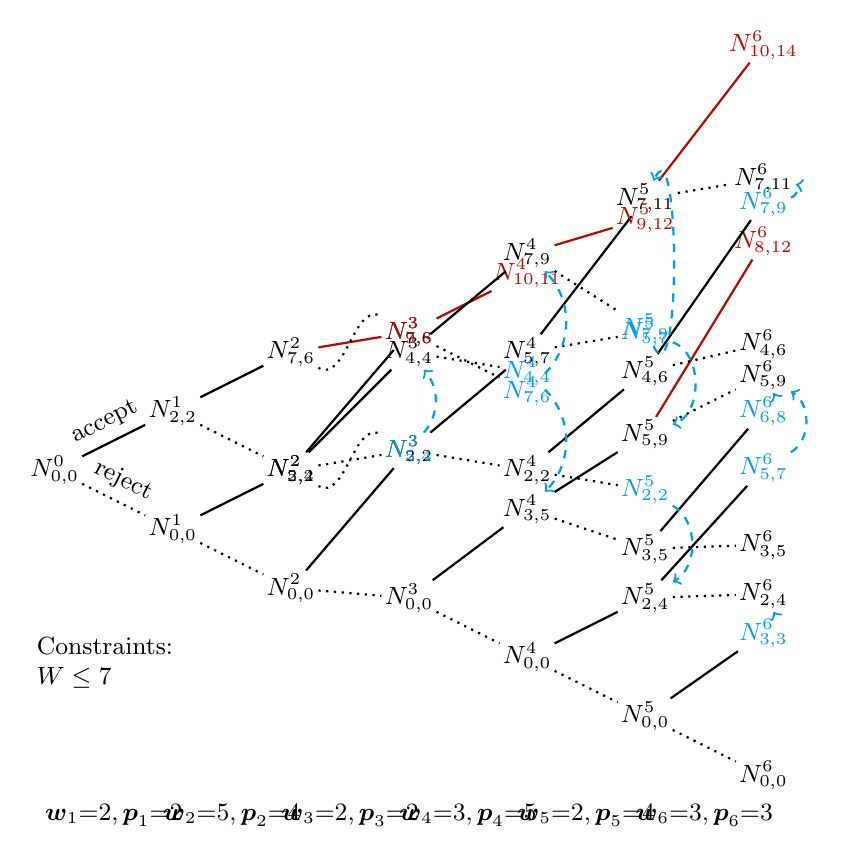
\begin{tikzpicture}[grow=right, sloped, font=\small]
    \node (N0w0p0) [state] {$N^0_{0,0}$}
    child {
        node (N1w0p0) [state] {$N^1_{0,0}$}
        child {
            node (N2w0p0) [state] {$N^2_{0,0}$}
            child {
                node (N3w0p0) [state, yshift=0.625cm] {$N^3_{0,0}$}
                child {
                    node (N4w0p0) [state] {$N^4_{0,0}$}
                    child {
                        node (N5w0p0) [state] {$N^5_{0,0}$}
                        child {
                            node (N6w0p0) [state] {$N^6_{0,0}$}
                            edge from parent [reject]
                        }
                        child {
                            node (N6w3p3) [state, dominated, yshift=0.3cm] {$N^6_{3,3}$}
                            edge from parent [accept]
                        }
                        edge from parent [reject]
                    }
                    child {
                        node (N5w2p4) [state] {$N^5_{2,4}$}
                        child {
                            node (N6w2p4) [state, yshift=0.8cm] {$N^6_{2,4}$}
                            edge from parent [reject]
                        }
                        child {
                            node (N6w5p7) [state, dominated, yshift=0.9cm] {$N^6_{5,7}$}
                            edge from parent [accept]
                        }
                        edge from parent [accept]
                    }
                    edge from parent [reject]
                }
                child {
                    node (N4w3p5) [state, yshift=0.375cm] {$N^4_{3,5}$}
                    child {
                        node (N5w3p5) [state, yshift=0.25cm] {$N^5_{3,5}$}
                        child {
                            node (N6w3p5) [state, yshift=0.8cm] {$N^6_{3,5}$}
                            edge from parent [reject]
                        }
                        child {
                            node (N6w6p8) [state, dominated, yshift=1cm] {$N^6_{6,8}$}
                            edge from parent [accept]
                        }
                        edge from parent [reject]
                    }
                    child {
                        node (N5w5p9) [state, yshift=0.2cm] {$N^5_{5,9}$}
                        child {
                            node (N6w5p9) [state, yshift=1.5cm] {$N^6_{5,9}$}
                            edge from parent [reject]
                        }
                        child {
                            node [state, infeasible, yshift=1.7cm] {$N^6_{8,12}$}
                            edge from parent [accept, infeasible]
                        }
                        edge from parent [accept]
                    }
                    edge from parent [accept]
                }
                edge from parent [reject]
            }
            child {
                node (N3w2p2) [state, yshift=1cm] {$N^3_{2,2}$}
                child {
                    node [state, yshift=0.5cm] {$N^4_{2,2}$}
                    child {
                        node (N5w2p2) [state, dominated, yshift=0.5cm] {$N^5_{2,2}$}
                        edge from parent [reject]
                    }
                    child {
                        node (N5w4p6) [state, yshift=0.5cm] {$N^5_{4,6}$}
                        child {
                            node [state, yshift=1.1cm] {$N^6_{4,6}$}
                            edge from parent [reject]
                        }
                        child {
                            node (N6w7p9) [state, dominated, yshift=1.4cm] {$N^6_{7,9}$}
                            edge from parent [accept]
                        }
                        edge from parent [accept]
                    }
                    edge from parent [reject]
                }
                child {
                    node [state, yshift=0.5cm] {$N^4_{5,7}$}
                    child {
                        node (N5w5p7) [state, dominated, yshift=1.0cm] {$N^5_{5,7}$}
                        edge from parent [reject]
                    }
                    child {
                        node (N5w7p11) [state, yshift=1.2cm] {$N^5_{7,11}$}
                        child {
                            node (N6w7p11) [state, yshift=1cm] {$N^6_{7,11}$}
                            edge from parent [reject]
                        }
                        child {
                            node [state, infeasible, yshift=1.2cm] {$N^6_{10,14}$}
                            edge from parent [accept, infeasible]
                        }
                        edge from parent [accept]
                    }
                    edge from parent [accept]
                }
                edge from parent [accept]
            }
            edge from parent [reject]
        }
        child {
            node (N2w5p5) [state] {$N^2_{5,4}$}
            child {
                node (N3w5p4) [state, dominated, yshift=1cm] {$N^3_{5,4}$}
                edge from parent [reject]
            }
            child {
                node (N3w7p6) [state, yshift=1cm] {$N^3_{7,6}$}
                child {
                    node (N4w7p6) [state, dominated] {$N^4_{7,6}$}
                    edge from parent [reject]
                }
                child {
                    node [state, infeasible] {$N^4_{10,11}$}
                    edge from parent [accept, infeasible]
                }
                edge from parent [accept]
            }
            edge from parent [accept]
        }
        edge from parent [reject] node [midway, above] { reject }
    }
    child {
        node [state] {$N^1_{2,2}$}
        child {
            node (N2w2p2) [state] {$N^2_{2,2}$}
            child {
                node (N3w4p4) [state, yshift=1.5cm] {$N^3_{4,4}$}
                child {
                    node (N4w4p4) [state, dominated, yshift=0.5cm] {$N^4_{4,4}$}
                    edge from parent [reject]
                }
                child {
                    node (N4w7p9) [state, yshift=0.5cm] {$N^4_{7,9}$}
                    child {
                        node (N5w7p9) [state, dominated, yshift=-0.2cm] {$N^5_{7,9}$}
                        edge from parent [reject]
                    }
                    child {
                        node (N5w9p12) [state, infeasible, yshift=-0.3cm] {$N^5_{9,12}$}
                        edge from parent [accept, infeasible]
                    }
                    edge from parent [accept]
                }
                edge from parent [accept]
            }
            edge from parent [reject]
        }
        child {
            node (N2w7p6) [state] {$N^2_{7,6}$}
            child {
                node [state, infeasible, yshift=0.25cm] {$N^3_{9,8}$}
                edge from parent [accept, infeasible]
            }
            edge from parent [accept]
        }
        edge from parent [accept] node [midway, above] { accept }
    };

    \coordinate (SC) at ($(N0w0p0.west)+(0cm,-2cm)$);
    \node [anchor=north west, text width=8em, visible on=<4->] at (SC) {Constraints:
    \\$W \le 7$};

    \coordinate (B1x) at ($(N0w0p0)!0.5!(N1w0p0)$);
    \coordinate (B1) at (B1x|-N6w0p0);
    \node [visible on=<2->, below=0.25cm of B1] {$\boldsymbol{w}_1{=}2, \boldsymbol{p}_1{=}2$};

    \coordinate (B2x) at ($(N1w0p0)!0.5!(N2w0p0)$);
    \coordinate (B2) at (B2x|-N6w0p0);
    \node [visible on=<3->, below=0.25cm of B2] {$\boldsymbol{w}_2{=}5, \boldsymbol{p}_2{=}4$};

    \coordinate (B3x) at ($(N2w0p0)!0.5!(N3w0p0)$);
    \coordinate (B3) at (B3x|-N6w0p0);
    \node [visible on=<4->, below=0.25cm of B3] {$\boldsymbol{w}_3{=}2, \boldsymbol{p}_3{=}2$};

    \coordinate (B4x) at ($(N3w0p0)!0.5!(N4w0p0)$);
    \coordinate (B4) at (B4x|-N6w0p0);
    \node [visible on=<5->, below=0.25cm of B4] {$\boldsymbol{w}_4{=}3, \boldsymbol{p}_4{=}5$};

    \coordinate (B5x) at ($(N4w0p0)!0.5!(N5w0p0)$);
    \coordinate (B5) at (B5x|-N6w0p0);
    \node [visible on=<6->, below=0.25cm of B5] {$\boldsymbol{w}_5{=}2, \boldsymbol{p}_5{=}4$};

    \coordinate (B6x) at ($(N5w0p0)!0.5!(N6w0p0)$);
    \coordinate (B6) at (B6x|-N6w0p0);
    \node [visible on=<7->, below=0.25cm of B6] {$\boldsymbol{w}_6{=}3, \boldsymbol{p}_6{=}3$};

    \draw [visible on=<4->, reject, out=330, in=150] (N2w2p2) to (N3w2p2);
    \draw [visible on=<4->, reject, out=330, in=150] (N2w7p6) to (N3w7p6);
    \draw [visible on=<4->, domination, out=50, in=310] (N3w5p4) to (N3w4p4);
    \draw [visible on=<5->, domination, out=45, in=315] (N4w7p6) to (N4w7p9);
    \draw [visible on=<5->, domination, out=315, in=45] (N4w4p4) to (N4w3p5);
    \draw [visible on=<6->, domination, out=295, in=65] (N5w7p9) to (N5w7p11);
    \draw [visible on=<6->, domination, out=340, in=20] (N5w5p7) to (N5w5p9);
    \draw [visible on=<6->, domination, out=330, in=30] (N5w2p2) to (N5w2p4);
    \draw [visible on=<7->, domination, out=10, in=350] (N6w7p9) to (N6w7p11);
    \draw [visible on=<7->, domination, out=30, in=330] (N6w5p7) to (N6w5p9);
    \draw [visible on=<7->, domination, out=60, in=300] (N6w3p3) to (N6w2p4);
    \draw [visible on=<7->, domination, out=60, in=300] (N6w6p8) to (N6w5p9);
\end{tikzpicture}
\end{nearlyplainframe}

\begin{frame}[t]{Is This Correct?}
    \begin{minipage}{0.4\paperwidth}
        Do you trust the theory?

        \bigskip

        \uncover<2->{Do you trust your PhD student to implement it correctly?}

        \bigskip

        \uncover<3->{Would you trust this inside a larger solver, where side constraints could
        apply?}
    \end{minipage}\hfill\begin{minipage}{0.4\paperwidth}%
        \uncover<4->{\centering
\includegraphics[width=0.3\paperwidth]{allofthethings.jpg}}
    \end{minipage}
\end{frame}

\begin{frame}{Knapsack as a Pseudo-Boolean Problem}
    \begin{align*}
        &2 x_1 + 5 x_2 + 2 x_3 + 3 x_4 + 2 x_5 + 3 x_6 \le 7 \\
        \text{maximise~} &2 x_1 + 4 x_2 + 2 x_3 + 5 x_4 + 4 x_5 + 3 x_6
    \end{align*}

    \bigskip

    We must \emph{describe} knapsack in pseudo-Boolean terms, but our solver can do
    whatever it likes.
\end{frame}

\begin{frame}{Proofs for Dynamic Programming Algorithms for Knapsack}
    \begin{itemize}
        \item For backtracking search, we constructed a proof tree out of RUP steps.
        \item For dynamic programming:
            \begin{itemize}
                \item Use extension variables to describe states.
                \item Prove implications between states to create a decision diagram.
            \end{itemize}
    \end{itemize}
\end{frame}

\begin{frame}{Extension Variables for States}
    For each state (or entry in the matrix) on layer $\ell$, create extension variables
    \begin{align*}
        W^{\ell}_{w} &\Leftrightarrow \sum_{i=1}^{\ell} \boldsymbol{w}_i x_i \ge w \\
        P^{\ell}_{p} &\Leftrightarrow \sum_{i=1}^{\ell} \boldsymbol{p}_i x_i \le p \\
        N^{\ell}_{w,p} & \Leftrightarrow W^{\ell}_{w} + P^{\ell}_{p} \ge 2
    \end{align*}
\end{frame}

\begin{frame}[t]{Transitioning Between States}
    \begin{minipage}[t]{0.3\framewidth}
    \uncover<1->{
        We don't have to take an item on layer $\ell$, so need to prove:
        \begin{align*}
            W^{\ell-1}_{w} \land \overline{x}_\ell &\Rightarrow W^\ell_\mathit{w} \\
            P^{\ell-1}_{p} \land \overline{x}_\ell &\Rightarrow P^\ell_\mathit{p} \\
            N^{\ell-1}_{w,p} \land \overline{x}_\ell &\Rightarrow N^\ell_{w,p}
        \end{align*}
    }
    \end{minipage}\hfill\begin{minipage}[t]{0.30\framewidth}
    \uncover<2->{
        If we can't take item on layer $\ell$, need to prove:
        \begin{align*}
            W^{\ell-1}_{w} &\Rightarrow \overline{x}_\ell \\
            N^{\ell-1}_{w,p} &\Rightarrow \overline{x}_\ell  \\
            N^{\ell-1}_{w,p} &\Rightarrow N^\ell_{w,p}
        \end{align*}
    }
    \end{minipage}\hfill\begin{minipage}[t]{0.35\framewidth}
    \uncover<3->{
        If we can take item on layer $\ell$, we need to prove:
        \begin{align*}
            W^{\ell-1}_{w} \land x_\ell &\Rightarrow W^\ell_{w'} \\
            P^{\ell-1}_{p} \land x_\ell &\Rightarrow P^\ell_{p'} \\
            N^{\ell-1}_{w,p} \land x_\ell &\Rightarrow N^\ell_{w',p'} \\
            N^{\ell-1}_{w,p} &\Rightarrow N^\ell_{w,p} + N^\ell_{w',p'} \ge 1
        \end{align*}
        where
        \begin{align*}
            (w', p') &= (w + \boldsymbol{w}_\ell, p + \boldsymbol{p}_\ell)
        \end{align*}
    }
    \end{minipage}
\end{frame}

\begin{frame}{Merged States}
    For each $N^\ell_{w,p}$ that is dominated by some other $N^\ell_{w',p'}$, we prove
        $N^\ell_{w,p} \Rightarrow N^\ell_{w',p'}$.

        \medskip

    We can do this by unwrapping the conjunction, proving
    \begin{align*}
        & W^\ell_{w} \Rightarrow W^\ell_{w'} & \text{i.e.} && (\sum_{i=1}^{\ell} \boldsymbol{w}_i
        x_i \ge w) \Rightarrow (\sum_{i=1}^{\ell} \boldsymbol{w}_i x_i \ge w') &\text{~for some~} w' \le w \\
        & P^\ell_{p} \Rightarrow P^\ell_{p'} & \text{i.e.} && (\sum_{i=1}^{\ell} \boldsymbol{p}_i
        x_i \ge p) \Rightarrow (\sum_{i=1}^{\ell} \boldsymbol{p}_i x_i \ge p') &\text{~for some~} p' \ge p \\
    \end{align*}
    ``If there is an assignment to the first $\ell$ $x_i$ variables where the weight sums to at
    least 7 and the profit to no more than 4, then there is an assignment where the weight sums
    to at least 6 and the profit to no more than 5''.
\end{frame}

\begin{frame}{Establishing Completeness}
    Must show that we have to be in one of the states on this layer,
    \begin{align*}
        \sum_{(w,p)~\text{on layer}~\ell} N^\ell_{w,p} \ge 1
    \end{align*}

    We can use the at-least-one constraint
    \begin{align*}
        \sum_{(w,p)~\text{on layer}~\ell - 1} N^{\ell-1}_{w,p} \ge 1
    \end{align*}
    from the previous layer, and resolve on each \begin{align*}
        N^{\ell-1}_{w,p} &\Rightarrow N^\ell_{w,p} + N^\ell_{w',p'} \ge 1 &&\text{or}&
        N^{\ell-1}_{w,p} &\Rightarrow N^\ell_{w,p}
    \end{align*}
\end{frame}

\begin{frame}{Reading Off a Conclusion}
    We can log an optimal solution, and get a solution-improving constraint.

    \bigskip

    We have an at-least-one constraint over feasible states on the final layer, which
    we can unwrap to only talk about profits.

    \bigskip

    The solution-improving constraint contradicts each entry in the at-least-one
    constraint.
\end{frame}

\section{Cool Things I Will Not Have Time For}

\subsection{Gocht, McCreesh, Nordstr\"om: An Auditable Constraint Programming Solver, CP 2022}

\begin{frame}{Autotabulation}
    \begin{itemize}
        \item Sometimes advantageous to replace several constraints over the same
            variables with a single table constraint.
        \item Can be done by a skilled modeller, or by a solver automatically.
            \begin{itemize}
                \item But what if the modeller or solver makes a mistake?
            \end{itemize}
        \item We can do this inside the proof, rather than inside the model.
    \end{itemize}
\end{frame}

\begin{frame}{Autotabulation Proofs}
    \begin{itemize}
        \item Run a search over a restricted subset of variables.
        \item Whenever we find a solution, create an extension variable \[
                t_i \Leftrightarrow (x_{{=}1} \land y_{{=}2} \land z_{{=}4})
            \]
        \item For the remainder of the proof, add $\overline{t}_i$ as a guess.
        \item End up deriving $\land_i \overline{t}_i \Rightarrow \bot$,
            which is $\lor_i t_i$ or $\sum_i t_i \ge 1$.
    \end{itemize}
\end{frame}

\subsection{Demirovi\'c, McCreesh, McIlree, Nordstr\"om, Oertel, Sidorov: Unpublished}

\begin{frame}{Knapsack as a Constraint}
    \begin{align*}
        &x_i \in \{0, 1, \text{maybe other non-negative values}\}\\
        &W, P \in \{\text{some domain of non-negative values}\}\\
        &W = \sum_i \boldsymbol{w}_i x_i\\
        &P = \sum_i \boldsymbol{p}_i x_i
    \end{align*}

    Now we can have lower and upper bounds on both $W$ and $P$, and maybe we can reason that some
    items must or must not be taken.

    \medskip

    Effectively we're solving two (or one, or more?) non-negative integer linear equations simultaneously.
\end{frame}

\begin{frame}{Decision Diagrams are Table Constraints but Better}
    \begin{itemize}
        \item Can often represent the solution set compactly as a decision diagram.
        \item Decision diagrams are like tables, but with bits of the table merged together.
    \end{itemize}
\end{frame}

\begin{frame}{A Change of States}
    For each state (or entry in the matrix) on layer $\ell$, define
    \begin{align*}
        W{\uparrow}^{\ell}_{w} &\Leftrightarrow \sum_{i=1}^{\ell} \boldsymbol{w}_i x_i \ge w
        &&\text{and}&
        W{\downarrow}^{\ell}_{w} &\Leftrightarrow \sum_{i=1}^{\ell} \boldsymbol{w}_i x_i \le w \\
        P{\uparrow}^{\ell}_{p} &\Leftrightarrow \sum_{i=1}^{\ell} \boldsymbol{p}_i x_i \ge p
        &&\text{and}&
        P{\downarrow}^{\ell}_{p} &\Leftrightarrow \sum_{i=1}^{\ell} \boldsymbol{p}_i x_i \le p
    \end{align*}\begin{align*}
        N^{\ell}_{w,p} & \Leftrightarrow W{\uparrow}^{\ell}_{w} + W{\downarrow}^{\ell}_{w} + P{\uparrow}^{\ell}_{p} + P{\downarrow}^{\ell}_{p} \ge 4
    \end{align*}
    So now our states represent \emph{exact} weights and profits.
\end{frame}

\begin{frame}{A Change of Merge Rules}
    We can no longer merge non-identical states!

    \bigskip

    Reassuringly, the proofs won't work if you try this\ldots

    \bigskip

    End up trying to prove ``if there is an assignment to the first $\ell$ $x_i$ variables where the weight sums to
    \emph{exactly} 7 and the profit to \emph{exactly} 4, then there is an assignment where the weight sums
    to \emph{exactly} 6 and the profit to \emph{exactly} 5.

\end{frame}

\begin{frame}{Establishing Arc Consistency}
    We can read off all possible values for $P$ and $W$ from the final layer.

    \bigskip

    Easy to use this and resolution with the at-least-one constraint to eliminate all
    other values.

    \bigskip

    If we used weaker state reification variables, we could merge more states but would get weaker
    consistency on the variables.

    \bigskip

    But what about the $x_i$ variables?
\end{frame}

\begin{nearlyplainframe}[t]{Forced and Forbidden Items}
\tikzstyle{level 1}=[level distance=2.20cm, sibling distance=4.00cm]
\tikzstyle{level 2}=[level distance=2.20cm, sibling distance=2.00cm]
\tikzstyle{level 3}=[level distance=2.20cm, sibling distance=1.00cm]
\tikzstyle{level 4}=[level distance=2.20cm, sibling distance=0.75cm]
\tikzstyle{level 5}=[level distance=2.20cm, sibling distance=0.50cm]
\tikzstyle{level 6}=[level distance=2.20cm, sibling distance=0.30cm]
\vspace*{-1cm}
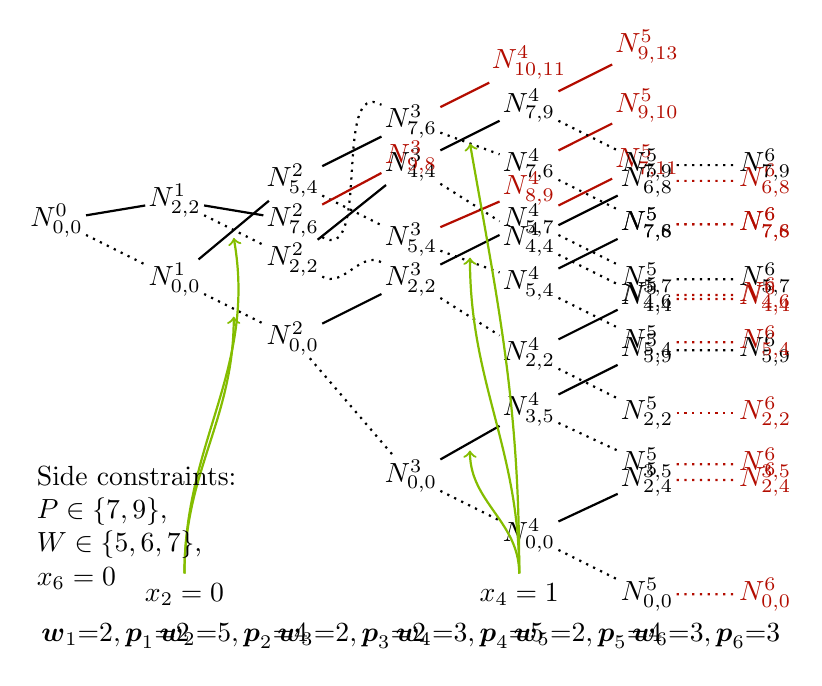
\begin{tikzpicture}[grow=right, sloped]
    \node (N0w0p0) [state, visible on=<1-7>] {$N^0_{0,0}$}
    child {
        node (N1w0p0) [state] {$N^1_{0,0}$}
        child {
            node (N2w0p0) [state] {$N^2_{0,0}$}
            child {
                node (N3w0p0) [state, yshift=-1.0cm] {$N^3_{0,0}$}
                child {
                    node (N4w0p0) [state, backwards, visible on=<1-3>] {$N^4_{0,0}$}
                    child {
                        node (N5w0p0) [state, backwards, visible on=<1-2>] {$N^5_{0,0}$}
                        child {
                            node (N6w0p0) [state, infeasible, visible on=<1>] {$N^6_{0,0}$}
                            edge from parent [reject, infeasible, visible on=<1>]
                        }
                        edge from parent [reject, backwards, visible on=<1-2>]
                    }
                    child {
                        node [state, backwards, visible on=<1-2>, yshift=-0.05cm] {$N^5_{2,4}$}
                        child {
                            node [state, infeasible, visible on=<1>] {$N^6_{2,4}$}
                            edge from parent [reject, infeasible, visible on=<1>]
                        }
                        edge from parent [accept, backwards, visible on=<1-2>]
                    }
                    edge from parent [reject, backwards, visible on=<1-3>]
                }
                child {
                    node [state, yshift=0.1cm] {$N^4_{3,5}$}
                    child {
                        node [state, backwards, visible on=<1-2>, yshift=0.05cm] {$N^5_{3,5}$}
                        child {
                            node [state, infeasible, visible on=<1>] {$N^6_{3,5}$}
                            edge from parent [reject, infeasible, visible on=<1>]
                        }
                        edge from parent [reject, backwards, visible on=<1-2>]
                    }
                    child {
                        node [state] {$N^5_{5,9}$}
                        child {
                            node [state] {$N^6_{5,9}$}
                            edge from parent [reject]
                        }
                        edge from parent [accept]
                    }
                    edge from parent [accept] coordinate (F4c) [midway]
                }
                edge from parent [reject]
            }
            child {
                node (N3w2p2) [state] {$N^3_{2,2}$}
                child {
                    node [state, backwards, visible on=<1-3>, yshift=-0.2cm] {$N^4_{2,2}$}
                    child {
                        node [state, backwards, visible on=<1-2>] {$N^5_{2,2}$}
                        child {
                            node [state, infeasible, visible on=<1>] {$N^6_{2,2}$}
                            edge from parent [reject, infeasible, visible on=<1>]
                        }
                        edge from parent [reject, backwards, visible on=<1-2>]
                    }
                    child {
                        node [state, backwards, visible on=<1-2>] {$N^5_{4,6}$}
                        child {
                            node [state, infeasible, visible on=<1>] {$N^6_{4,6}$}
                            edge from parent [reject, infeasible, visible on=<1>]
                        }
                        edge from parent [accept, backwards, visible on=<1-2>]
                    }
                    edge from parent [reject, backwards, visible on=<1-3>]
                }
                child {
                    node [state] {$N^4_{5,7}$}
                    child {
                        node [state] {$N^5_{5,7}$}
                        child {
                            node [state] {$N^6_{5,7}$}
                            edge from parent [reject]
                        }
                        edge from parent [reject]
                    }
                    child {
                        node [state, infeasible, visible on=<1>] {$N^5_{7,11}$}
                        edge from parent [accept, infeasible, visible on=<1>]
                    }
                    edge from parent [accept] coordinate (F4b) [midway]
                }
                edge from parent [accept]
            }
            edge from parent [reject] coordinate (F2b) [midway]
        }
        child {
            node (N2w5p5) [state, backwards, visible on=<1-5>, yshift=0.5cm] {$N^2_{5,4}$}
            child {
                node [state, backwards, visible on=<1-4>] {$N^3_{5,4}$}
                child {
                    node [state, backwards, visible on=<1-3>, yshift=0.2cm] {$N^4_{5,4}$}
                    child {
                        node [state, backwards, visible on=<1-2>] {$N^5_{5,4}$}
                        child {
                            node [state, infeasible, visible on=<1>] {$N^6_{5,4}$}
                            edge from parent [reject, infeasible, visible on=<1>]
                        }
                        edge from parent [reject, backwards, visible on=<1-2>]
                    }
                    child {
                        node [state, backwards, visible on=<1-2>] {$N^5_{7,8}$}
                        child {
                            node [state, infeasible, visible on=<1>] {$N^6_{7,8}$}
                            edge from parent [reject, infeasible, visible on=<1>]
                        }
                        edge from parent [accept, backwards, visible on=<1-2>]
                    }
                    edge from parent [reject, backwards, visible on=<1-3>]
                }
                child {
                    node [state, infeasible, visible on=<1>, yshift=-0.1cm] {$N^4_{8,9}$}
                    edge from parent [accept, infeasible, visible on=<1>]
                }
                edge from parent [reject, backwards, visible on=<1-4>]
            }
            child {
                node (N3w7p6) [state, backwards, visible on=<1-4>] {$N^3_{7,6}$}
                child {
                    node [state, backwards, visible on=<1-3>, yshift=0.2cm] {$N^4_{7,6}$}
                    child {
                        node [state, backwards, visible on=<1-2>] {$N^5_{7,6}$}
                        child {
                            node [state, infeasible, visible on=<1>] {$N^6_{7,6}$}
                            edge from parent [reject, infeasible, visible on=<1>]
                        }
                        edge from parent [reject, backwards, visible on=<1-2>]
                    }
                    child {
                        node [state, infeasible, visible on=<1>] {$N^5_{9,10}$}
                        edge from parent [accept, infeasible, visible on=<1>]
                    }
                    edge from parent [reject, backwards, visible on=<1-3>]
                }
                child {
                    node [state, infeasible, visible on=<1>] {$N^4_{10,11}$}
                    edge from parent [accept, infeasible, visible on=<1>]
                }
                edge from parent [accept, backwards, visible on=<1-4>]
            }
            edge from parent [accept, backwards, visible on=<1-5>]
        }
        edge from parent [reject]
    }
    child {
        node [state, yshift=-0.5cm] {$N^1_{2,2}$}
        child {
            node (N2w2p2) [state] {$N^2_{2,2}$}
            child {
                node [state, yshift=1.2cm] {$N^3_{4,4}$}
                child {
                    node [state, backwards, visible on=<1-3>, yshift=-0.2cm] {$N^4_{4,4}$}
                    child {
                        node [state, backwards, visible on=<1-2>] {$N^5_{4,4}$}
                        child {
                            node [state, infeasible, visible on=<1>] {$N^6_{4,4}$}
                            edge from parent [reject, infeasible, visible on=<1>]
                        }
                        edge from parent [reject, backwards, visible on=<1-2>]
                    }
                    child {
                        node [state, backwards, visible on=<1-2>] {$N^5_{6,8}$}
                        child {
                            node [state, infeasible, visible on=<1>] {$N^6_{6,8}$}
                            edge from parent [reject, infeasible, visible on=<1>]
                        }
                        edge from parent [accept, visible on=<1-2>]
                    }
                    edge from parent [reject, backwards, visible on=<1-3>]
                }
                child {
                    node [state] {$N^4_{7,9}$}
                    child {
                        node [state] {$N^5_{7,9}$}
                        child {
                            node [state] {$N^6_{7,9}$}
                            edge from parent [reject]
                        }
                        edge from parent [reject]
                    }
                    child {
                        node [state, infeasible, visible on=<1>] {$N^5_{9,13}$}
                        edge from parent [accept, infeasible, visible on=<1>]
                    }
                    edge from parent [accept] coordinate (F4a) [midway]
                }
                edge from parent [accept]
            }
            edge from parent [reject] coordinate (F2a) [midway]
        }
        child {
            node (N2w7p6) [state, backwards, visible on=<1-5>, yshift=-1cm] {$N^2_{7,6}$}
            child {
                node [state, infeasible, visible on=<1>, yshift=0.8cm] {$N^3_{9,8}$}
                edge from parent [accept, infeasible, visible on=<1>]
            }
            edge from parent [accept, backwards, visible on=<1-5>]
        }
        edge from parent [accept]
    };

    \draw [reject, out=330, in=150] (N2w2p2) to (N3w2p2);
    \draw [reject, backwards, out=330, in=150, visible on=<1-4>] (N2w7p6) to (N3w7p6);

    \coordinate (B1x) at ($(N0w0p0)!0.5!(N1w0p0)$);
    \coordinate (B1) at (B1x|-N6w0p0);
    \node [below=0.25cm of B1] {$\boldsymbol{w}_1{=}2, \boldsymbol{p}_1{=}2$};

    \coordinate (B2x) at ($(N1w0p0)!0.5!(N2w0p0)$);
    \coordinate (B2) at (B2x|-N6w0p0);
    \node [below=0.25cm of B2] {$\boldsymbol{w}_2{=}5, \boldsymbol{p}_2{=}4$};

    \coordinate (B3x) at ($(N2w0p0)!0.5!(N3w0p0)$);
    \coordinate (B3) at (B3x|-N6w0p0);
    \node [below=0.25cm of B3] {$\boldsymbol{w}_3{=}2, \boldsymbol{p}_3{=}2$};

    \coordinate (B4x) at ($(N3w0p0)!0.5!(N4w0p0)$);
    \coordinate (B4) at (B4x|-N6w0p0);
    \node [below=0.25cm of B4] {$\boldsymbol{w}_4{=}3, \boldsymbol{p}_4{=}5$};

    \coordinate (B5x) at ($(N4w0p0)!0.5!(N5w0p0)$);
    \coordinate (B5) at (B5x|-N6w0p0);
    \node [below=0.25cm of B5] {$\boldsymbol{w}_5{=}2, \boldsymbol{p}_5{=}4$};

    \coordinate (B6x) at ($(N5w0p0)!0.5!(N6w0p0)$);
    \coordinate (B6) at (B6x|-N6w0p0);
    \node [below=0.25cm of B6] {$\boldsymbol{w}_6{=}3, \boldsymbol{p}_6{=}3$};

    \node [visible on=<7>, left=0.0cm of B2] (x2) {$x_2=0$};
    \draw [->, visible on=<7>, color=uofglawn, thick] (x2) to[out=90, in=280] ($(F2a)+(0cm,-0.1cm)$);
    \draw [->, visible on=<7>, color=uofglawn, thick] (x2) to[out=90, in=270] ($(F2b)+(0cm,-0.1cm)$);

    \node [visible on=<7>, right=0.0cm of B4] (x4) {$x_4=1$};
    \draw [->, visible on=<7>, color=uofglawn, thick] (x4) to[out=90, in=280] ($(F4a)+(0cm,-0.1cm)$);
    \draw [->, visible on=<7>, color=uofglawn, thick] (x4) to[out=90, in=270] ($(F4b)+(0cm,-0.1cm)$);
    \draw [->, visible on=<7>, color=uofglawn, thick] (x4) to[out=90, in=270] ($(F4c)+(0cm,-0.1cm)$);

    \coordinate (SC) at ($(N0w0p0.west)+(0cm,-3cm)$);
    \node [anchor=north west, text width=8em] at (SC) {Side constraints:
    \\$P \in \{7, 9\}$,
    \\$W \in \{5, 6, 7\}$,
    \\$x_6 = 0$};
\end{tikzpicture}
\end{nearlyplainframe}

\section{Conclusion}

\begin{frame}{Solving and Justification Languages are Different}
    \begin{itemize}
        \item Traditional SAT view: solvers are searching for proofs, and there is a proof system
            that is ``natural'' for the description of the problem.
            \begin{itemize}
        \item <2-> A huge coincidence due to CDCL and the proof that SAT solvers can't count.
        \item <2-> Not really what's happening: there are resolution proofs that SAT solvers can't
            find.
            \end{itemize}
        \item <3-> We need a stronger input language and proof system to justify modern SAT solving techniques.
        \item <3-> A simpler input language and proof system is fine for justifying modern CP and graph solving
            techniques.
    \end{itemize}
\end{frame}

{
    \usebackgroundtemplate{
        \tikz[overlay, remember picture]
        \node[at=(current page.south), anchor=south, yshift=-1cm, inner sep=0pt]{\includegraphics[keepaspectratio=true, width=\paperwidth]{../../images/background2.jpg}};
    }

    \begin{frame}[plain,noframenumbering]
        \begin{tikzpicture}[remember picture, overlay]
            \node at (current page.north west) {
                \begin{tikzpicture}[remember picture, overlay]
                    \fill [fill=uofguniversityblue, anchor=north west] (0, 0) rectangle (\paperwidth, -2.8cm);
                \end{tikzpicture}
            };

            \node (logo) [anchor=north east, shift={(-0.8cm,-0.2cm)}] at (current page.north east) {
                
\includegraphics[keepaspectratio=true,scale=0.5]{../../images/UoG_keyline.pdf}
            };

            \node (logo2) [anchor=north, below=0.2cm of logo.south] {
                
\includegraphics[keepaspectratio=true,scale=0.1]{../../images/RAEngWhite.pdf}
            };

            \coordinate (logos) at ($(logo.south)!0.5!(logo2.north)$);

            \node [anchor=west, xshift=0.8cm] at (current page.west |- logos) {
                \begin{minipage}{0.60\paperwidth}\raggedright
                    \textcolor{white}{\url{https://ciaranm.github.io/}} \\[0.3cm]
                    \textcolor{white}{\href{mailto:ciaran.mccreesh@glasgow.ac.uk}{\nolinkurl{ciaran.mccreesh@glasgow.ac.uk}}}
                \end{minipage}
            };
        \end{tikzpicture}
    \end{frame}
}

\end{document}

